\documentclass{article} % For LaTeX2e
\usepackage{iclr2020_conference,times}

% Optional math commands from https://github.com/goodfeli/dlbook_notation.
%%%%% NEW MATH DEFINITIONS %%%%%

\usepackage{amsmath,amsfonts,bm}

% Mark sections of captions for referring to divisions of figures
\newcommand{\figleft}{{\em (Left)}}
\newcommand{\figcenter}{{\em (Center)}}
\newcommand{\figright}{{\em (Right)}}
\newcommand{\figtop}{{\em (Top)}}
\newcommand{\figbottom}{{\em (Bottom)}}
\newcommand{\captiona}{{\em (a)}}
\newcommand{\captionb}{{\em (b)}}
\newcommand{\captionc}{{\em (c)}}
\newcommand{\captiond}{{\em (d)}}

% Highlight a newly defined term
\newcommand{\newterm}[1]{{\bf #1}}


% Figure reference, lower-case.
\def\figref#1{figure~\ref{#1}}
% Figure reference, capital. For start of sentence
\def\Figref#1{Figure~\ref{#1}}
\def\twofigref#1#2{figures \ref{#1} and \ref{#2}}
\def\quadfigref#1#2#3#4{figures \ref{#1}, \ref{#2}, \ref{#3} and \ref{#4}}
% Section reference, lower-case.
\def\secref#1{section~\ref{#1}}
% Section reference, capital.
\def\Secref#1{Section~\ref{#1}}
% Reference to two sections.
\def\twosecrefs#1#2{sections \ref{#1} and \ref{#2}}
% Reference to three sections.
\def\secrefs#1#2#3{sections \ref{#1}, \ref{#2} and \ref{#3}}
% Reference to an equation, lower-case.
\def\eqref#1{equation~\ref{#1}}
% Reference to an equation, upper case
\def\Eqref#1{Equation~\ref{#1}}
% A raw reference to an equation---avoid using if possible
\def\plaineqref#1{\ref{#1}}
% Reference to a chapter, lower-case.
\def\chapref#1{chapter~\ref{#1}}
% Reference to an equation, upper case.
\def\Chapref#1{Chapter~\ref{#1}}
% Reference to a range of chapters
\def\rangechapref#1#2{chapters\ref{#1}--\ref{#2}}
% Reference to an algorithm, lower-case.
\def\algref#1{algorithm~\ref{#1}}
% Reference to an algorithm, upper case.
\def\Algref#1{Algorithm~\ref{#1}}
\def\twoalgref#1#2{algorithms \ref{#1} and \ref{#2}}
\def\Twoalgref#1#2{Algorithms \ref{#1} and \ref{#2}}
% Reference to a part, lower case
\def\partref#1{part~\ref{#1}}
% Reference to a part, upper case
\def\Partref#1{Part~\ref{#1}}
\def\twopartref#1#2{parts \ref{#1} and \ref{#2}}

\def\ceil#1{\lceil #1 \rceil}
\def\floor#1{\lfloor #1 \rfloor}
\def\1{\bm{1}}
\newcommand{\train}{\mathcal{D}}
\newcommand{\valid}{\mathcal{D_{\mathrm{valid}}}}
\newcommand{\test}{\mathcal{D_{\mathrm{test}}}}

\def\eps{{\epsilon}}


% Random variables
\def\reta{{\textnormal{$\eta$}}}
\def\ra{{\textnormal{a}}}
\def\rb{{\textnormal{b}}}
\def\rc{{\textnormal{c}}}
\def\rd{{\textnormal{d}}}
\def\re{{\textnormal{e}}}
\def\rf{{\textnormal{f}}}
\def\rg{{\textnormal{g}}}
\def\rh{{\textnormal{h}}}
\def\ri{{\textnormal{i}}}
\def\rj{{\textnormal{j}}}
\def\rk{{\textnormal{k}}}
\def\rl{{\textnormal{l}}}
% rm is already a command, just don't name any random variables m
\def\rn{{\textnormal{n}}}
\def\ro{{\textnormal{o}}}
\def\rp{{\textnormal{p}}}
\def\rq{{\textnormal{q}}}
\def\rr{{\textnormal{r}}}
\def\rs{{\textnormal{s}}}
\def\rt{{\textnormal{t}}}
\def\ru{{\textnormal{u}}}
\def\rv{{\textnormal{v}}}
\def\rw{{\textnormal{w}}}
\def\rx{{\textnormal{x}}}
\def\ry{{\textnormal{y}}}
\def\rz{{\textnormal{z}}}

% Random vectors
\def\rvepsilon{{\mathbf{\epsilon}}}
\def\rvtheta{{\mathbf{\theta}}}
\def\rva{{\mathbf{a}}}
\def\rvb{{\mathbf{b}}}
\def\rvc{{\mathbf{c}}}
\def\rvd{{\mathbf{d}}}
\def\rve{{\mathbf{e}}}
\def\rvf{{\mathbf{f}}}
\def\rvg{{\mathbf{g}}}
\def\rvh{{\mathbf{h}}}
\def\rvu{{\mathbf{i}}}
\def\rvj{{\mathbf{j}}}
\def\rvk{{\mathbf{k}}}
\def\rvl{{\mathbf{l}}}
\def\rvm{{\mathbf{m}}}
\def\rvn{{\mathbf{n}}}
\def\rvo{{\mathbf{o}}}
\def\rvp{{\mathbf{p}}}
\def\rvq{{\mathbf{q}}}
\def\rvr{{\mathbf{r}}}
\def\rvs{{\mathbf{s}}}
\def\rvt{{\mathbf{t}}}
\def\rvu{{\mathbf{u}}}
\def\rvv{{\mathbf{v}}}
\def\rvw{{\mathbf{w}}}
\def\rvx{{\mathbf{x}}}
\def\rvy{{\mathbf{y}}}
\def\rvz{{\mathbf{z}}}

% Elements of random vectors
\def\erva{{\textnormal{a}}}
\def\ervb{{\textnormal{b}}}
\def\ervc{{\textnormal{c}}}
\def\ervd{{\textnormal{d}}}
\def\erve{{\textnormal{e}}}
\def\ervf{{\textnormal{f}}}
\def\ervg{{\textnormal{g}}}
\def\ervh{{\textnormal{h}}}
\def\ervi{{\textnormal{i}}}
\def\ervj{{\textnormal{j}}}
\def\ervk{{\textnormal{k}}}
\def\ervl{{\textnormal{l}}}
\def\ervm{{\textnormal{m}}}
\def\ervn{{\textnormal{n}}}
\def\ervo{{\textnormal{o}}}
\def\ervp{{\textnormal{p}}}
\def\ervq{{\textnormal{q}}}
\def\ervr{{\textnormal{r}}}
\def\ervs{{\textnormal{s}}}
\def\ervt{{\textnormal{t}}}
\def\ervu{{\textnormal{u}}}
\def\ervv{{\textnormal{v}}}
\def\ervw{{\textnormal{w}}}
\def\ervx{{\textnormal{x}}}
\def\ervy{{\textnormal{y}}}
\def\ervz{{\textnormal{z}}}

% Random matrices
\def\rmA{{\mathbf{A}}}
\def\rmB{{\mathbf{B}}}
\def\rmC{{\mathbf{C}}}
\def\rmD{{\mathbf{D}}}
\def\rmE{{\mathbf{E}}}
\def\rmF{{\mathbf{F}}}
\def\rmG{{\mathbf{G}}}
\def\rmH{{\mathbf{H}}}
\def\rmI{{\mathbf{I}}}
\def\rmJ{{\mathbf{J}}}
\def\rmK{{\mathbf{K}}}
\def\rmL{{\mathbf{L}}}
\def\rmM{{\mathbf{M}}}
\def\rmN{{\mathbf{N}}}
\def\rmO{{\mathbf{O}}}
\def\rmP{{\mathbf{P}}}
\def\rmQ{{\mathbf{Q}}}
\def\rmR{{\mathbf{R}}}
\def\rmS{{\mathbf{S}}}
\def\rmT{{\mathbf{T}}}
\def\rmU{{\mathbf{U}}}
\def\rmV{{\mathbf{V}}}
\def\rmW{{\mathbf{W}}}
\def\rmX{{\mathbf{X}}}
\def\rmY{{\mathbf{Y}}}
\def\rmZ{{\mathbf{Z}}}

% Elements of random matrices
\def\ermA{{\textnormal{A}}}
\def\ermB{{\textnormal{B}}}
\def\ermC{{\textnormal{C}}}
\def\ermD{{\textnormal{D}}}
\def\ermE{{\textnormal{E}}}
\def\ermF{{\textnormal{F}}}
\def\ermG{{\textnormal{G}}}
\def\ermH{{\textnormal{H}}}
\def\ermI{{\textnormal{I}}}
\def\ermJ{{\textnormal{J}}}
\def\ermK{{\textnormal{K}}}
\def\ermL{{\textnormal{L}}}
\def\ermM{{\textnormal{M}}}
\def\ermN{{\textnormal{N}}}
\def\ermO{{\textnormal{O}}}
\def\ermP{{\textnormal{P}}}
\def\ermQ{{\textnormal{Q}}}
\def\ermR{{\textnormal{R}}}
\def\ermS{{\textnormal{S}}}
\def\ermT{{\textnormal{T}}}
\def\ermU{{\textnormal{U}}}
\def\ermV{{\textnormal{V}}}
\def\ermW{{\textnormal{W}}}
\def\ermX{{\textnormal{X}}}
\def\ermY{{\textnormal{Y}}}
\def\ermZ{{\textnormal{Z}}}

% Vectors
\def\vzero{{\bm{0}}}
\def\vone{{\bm{1}}}
\def\vmu{{\bm{\mu}}}
\def\vtheta{{\bm{\theta}}}
\def\va{{\bm{a}}}
\def\vb{{\bm{b}}}
\def\vc{{\bm{c}}}
\def\vd{{\bm{d}}}
\def\ve{{\bm{e}}}
\def\vf{{\bm{f}}}
\def\vg{{\bm{g}}}
\def\vh{{\bm{h}}}
\def\vi{{\bm{i}}}
\def\vj{{\bm{j}}}
\def\vk{{\bm{k}}}
\def\vl{{\bm{l}}}
\def\vm{{\bm{m}}}
\def\vn{{\bm{n}}}
\def\vo{{\bm{o}}}
\def\vp{{\bm{p}}}
\def\vq{{\bm{q}}}
\def\vr{{\bm{r}}}
\def\vs{{\bm{s}}}
\def\vt{{\bm{t}}}
\def\vu{{\bm{u}}}
\def\vv{{\bm{v}}}
\def\vw{{\bm{w}}}
\def\vx{{\bm{x}}}
\def\vy{{\bm{y}}}
\def\vz{{\bm{z}}}

% Elements of vectors
\def\evalpha{{\alpha}}
\def\evbeta{{\beta}}
\def\evepsilon{{\epsilon}}
\def\evlambda{{\lambda}}
\def\evomega{{\omega}}
\def\evmu{{\mu}}
\def\evpsi{{\psi}}
\def\evsigma{{\sigma}}
\def\evtheta{{\theta}}
\def\eva{{a}}
\def\evb{{b}}
\def\evc{{c}}
\def\evd{{d}}
\def\eve{{e}}
\def\evf{{f}}
\def\evg{{g}}
\def\evh{{h}}
\def\evi{{i}}
\def\evj{{j}}
\def\evk{{k}}
\def\evl{{l}}
\def\evm{{m}}
\def\evn{{n}}
\def\evo{{o}}
\def\evp{{p}}
\def\evq{{q}}
\def\evr{{r}}
\def\evs{{s}}
\def\evt{{t}}
\def\evu{{u}}
\def\evv{{v}}
\def\evw{{w}}
\def\evx{{x}}
\def\evy{{y}}
\def\evz{{z}}

% Matrix
\def\mA{{\bm{A}}}
\def\mB{{\bm{B}}}
\def\mC{{\bm{C}}}
\def\mD{{\bm{D}}}
\def\mE{{\bm{E}}}
\def\mF{{\bm{F}}}
\def\mG{{\bm{G}}}
\def\mH{{\bm{H}}}
\def\mI{{\bm{I}}}
\def\mJ{{\bm{J}}}
\def\mK{{\bm{K}}}
\def\mL{{\bm{L}}}
\def\mM{{\bm{M}}}
\def\mN{{\bm{N}}}
\def\mO{{\bm{O}}}
\def\mP{{\bm{P}}}
\def\mQ{{\bm{Q}}}
\def\mR{{\bm{R}}}
\def\mS{{\bm{S}}}
\def\mT{{\bm{T}}}
\def\mU{{\bm{U}}}
\def\mV{{\bm{V}}}
\def\mW{{\bm{W}}}
\def\mX{{\bm{X}}}
\def\mY{{\bm{Y}}}
\def\mZ{{\bm{Z}}}
\def\mBeta{{\bm{\beta}}}
\def\mPhi{{\bm{\Phi}}}
\def\mLambda{{\bm{\Lambda}}}
\def\mSigma{{\bm{\Sigma}}}

% Tensor
\DeclareMathAlphabet{\mathsfit}{\encodingdefault}{\sfdefault}{m}{sl}
\SetMathAlphabet{\mathsfit}{bold}{\encodingdefault}{\sfdefault}{bx}{n}
\newcommand{\tens}[1]{\bm{\mathsfit{#1}}}
\def\tA{{\tens{A}}}
\def\tB{{\tens{B}}}
\def\tC{{\tens{C}}}
\def\tD{{\tens{D}}}
\def\tE{{\tens{E}}}
\def\tF{{\tens{F}}}
\def\tG{{\tens{G}}}
\def\tH{{\tens{H}}}
\def\tI{{\tens{I}}}
\def\tJ{{\tens{J}}}
\def\tK{{\tens{K}}}
\def\tL{{\tens{L}}}
\def\tM{{\tens{M}}}
\def\tN{{\tens{N}}}
\def\tO{{\tens{O}}}
\def\tP{{\tens{P}}}
\def\tQ{{\tens{Q}}}
\def\tR{{\tens{R}}}
\def\tS{{\tens{S}}}
\def\tT{{\tens{T}}}
\def\tU{{\tens{U}}}
\def\tV{{\tens{V}}}
\def\tW{{\tens{W}}}
\def\tX{{\tens{X}}}
\def\tY{{\tens{Y}}}
\def\tZ{{\tens{Z}}}


% Graph
\def\gA{{\mathcal{A}}}
\def\gB{{\mathcal{B}}}
\def\gC{{\mathcal{C}}}
\def\gD{{\mathcal{D}}}
\def\gE{{\mathcal{E}}}
\def\gF{{\mathcal{F}}}
\def\gG{{\mathcal{G}}}
\def\gH{{\mathcal{H}}}
\def\gI{{\mathcal{I}}}
\def\gJ{{\mathcal{J}}}
\def\gK{{\mathcal{K}}}
\def\gL{{\mathcal{L}}}
\def\gM{{\mathcal{M}}}
\def\gN{{\mathcal{N}}}
\def\gO{{\mathcal{O}}}
\def\gP{{\mathcal{P}}}
\def\gQ{{\mathcal{Q}}}
\def\gR{{\mathcal{R}}}
\def\gS{{\mathcal{S}}}
\def\gT{{\mathcal{T}}}
\def\gU{{\mathcal{U}}}
\def\gV{{\mathcal{V}}}
\def\gW{{\mathcal{W}}}
\def\gX{{\mathcal{X}}}
\def\gY{{\mathcal{Y}}}
\def\gZ{{\mathcal{Z}}}

% Sets
\def\sA{{\mathbb{A}}}
\def\sB{{\mathbb{B}}}
\def\sC{{\mathbb{C}}}
\def\sD{{\mathbb{D}}}
% Don't use a set called E, because this would be the same as our symbol
% for expectation.
\def\sF{{\mathbb{F}}}
\def\sG{{\mathbb{G}}}
\def\sH{{\mathbb{H}}}
\def\sI{{\mathbb{I}}}
\def\sJ{{\mathbb{J}}}
\def\sK{{\mathbb{K}}}
\def\sL{{\mathbb{L}}}
\def\sM{{\mathbb{M}}}
\def\sN{{\mathbb{N}}}
\def\sO{{\mathbb{O}}}
\def\sP{{\mathbb{P}}}
\def\sQ{{\mathbb{Q}}}
\def\sR{{\mathbb{R}}}
\def\sS{{\mathbb{S}}}
\def\sT{{\mathbb{T}}}
\def\sU{{\mathbb{U}}}
\def\sV{{\mathbb{V}}}
\def\sW{{\mathbb{W}}}
\def\sX{{\mathbb{X}}}
\def\sY{{\mathbb{Y}}}
\def\sZ{{\mathbb{Z}}}

% Entries of a matrix
\def\emLambda{{\Lambda}}
\def\emA{{A}}
\def\emB{{B}}
\def\emC{{C}}
\def\emD{{D}}
\def\emE{{E}}
\def\emF{{F}}
\def\emG{{G}}
\def\emH{{H}}
\def\emI{{I}}
\def\emJ{{J}}
\def\emK{{K}}
\def\emL{{L}}
\def\emM{{M}}
\def\emN{{N}}
\def\emO{{O}}
\def\emP{{P}}
\def\emQ{{Q}}
\def\emR{{R}}
\def\emS{{S}}
\def\emT{{T}}
\def\emU{{U}}
\def\emV{{V}}
\def\emW{{W}}
\def\emX{{X}}
\def\emY{{Y}}
\def\emZ{{Z}}
\def\emSigma{{\Sigma}}

% entries of a tensor
% Same font as tensor, without \bm wrapper
\newcommand{\etens}[1]{\mathsfit{#1}}
\def\etLambda{{\etens{\Lambda}}}
\def\etA{{\etens{A}}}
\def\etB{{\etens{B}}}
\def\etC{{\etens{C}}}
\def\etD{{\etens{D}}}
\def\etE{{\etens{E}}}
\def\etF{{\etens{F}}}
\def\etG{{\etens{G}}}
\def\etH{{\etens{H}}}
\def\etI{{\etens{I}}}
\def\etJ{{\etens{J}}}
\def\etK{{\etens{K}}}
\def\etL{{\etens{L}}}
\def\etM{{\etens{M}}}
\def\etN{{\etens{N}}}
\def\etO{{\etens{O}}}
\def\etP{{\etens{P}}}
\def\etQ{{\etens{Q}}}
\def\etR{{\etens{R}}}
\def\etS{{\etens{S}}}
\def\etT{{\etens{T}}}
\def\etU{{\etens{U}}}
\def\etV{{\etens{V}}}
\def\etW{{\etens{W}}}
\def\etX{{\etens{X}}}
\def\etY{{\etens{Y}}}
\def\etZ{{\etens{Z}}}

% The true underlying data generating distribution
\newcommand{\pdata}{p_{\rm{data}}}
% The empirical distribution defined by the training set
\newcommand{\ptrain}{\hat{p}_{\rm{data}}}
\newcommand{\Ptrain}{\hat{P}_{\rm{data}}}
% The model distribution
\newcommand{\pmodel}{p_{\rm{model}}}
\newcommand{\Pmodel}{P_{\rm{model}}}
\newcommand{\ptildemodel}{\tilde{p}_{\rm{model}}}
% Stochastic autoencoder distributions
\newcommand{\pencode}{p_{\rm{encoder}}}
\newcommand{\pdecode}{p_{\rm{decoder}}}
\newcommand{\precons}{p_{\rm{reconstruct}}}

\newcommand{\laplace}{\mathrm{Laplace}} % Laplace distribution

\newcommand{\E}{\mathbb{E}}
\newcommand{\Ls}{\mathcal{L}}
\newcommand{\R}{\mathbb{R}}
\newcommand{\emp}{\tilde{p}}
\newcommand{\lr}{\alpha}
\newcommand{\reg}{\lambda}
\newcommand{\rect}{\mathrm{rectifier}}
\newcommand{\softmax}{\mathrm{softmax}}
\newcommand{\sigmoid}{\sigma}
\newcommand{\softplus}{\zeta}
\newcommand{\KL}{D_{\mathrm{KL}}}
\newcommand{\Var}{\mathrm{Var}}
\newcommand{\standarderror}{\mathrm{SE}}
\newcommand{\Cov}{\mathrm{Cov}}
% Wolfram Mathworld says $L^2$ is for function spaces and $\ell^2$ is for vectors
% But then they seem to use $L^2$ for vectors throughout the site, and so does
% wikipedia.
\newcommand{\normlzero}{L^0}
\newcommand{\normlone}{L^1}
\newcommand{\normltwo}{L^2}
\newcommand{\normlp}{L^p}
\newcommand{\normmax}{L^\infty}

\newcommand{\parents}{Pa} % See usage in notation.tex. Chosen to match Daphne's book.

\DeclareMathOperator*{\argmax}{arg\,max}
\DeclareMathOperator*{\argmin}{arg\,min}

\DeclareMathOperator{\sign}{sign}
\DeclareMathOperator{\Tr}{Tr}
\let\ab\allowbreak


\usepackage{hyperref}
\usepackage{url}

\usepackage{amsmath}
\usepackage{amssymb}
\usepackage{wasysym}
\usepackage{amsthm}
\usepackage{graphicx}

\newtheorem{theorem}{Theorem}[section]
\newtheorem{definition}{Definition}[section]
\newtheorem{lemma}[theorem]{Lemma}
\newtheorem{proposition}[theorem]{Proposition}
\newtheorem{corollary}[theorem]{Corollary}
\newtheorem{assumption}[definition]{Assumption}
\newtheorem{conjecture}[theorem]{Conjecture}
\newtheorem{remark}[theorem]{Remark}


\title{Global graph curvature}

% Authors must not appear in the submitted version. They should be hidden
% as long as the \iclrfinalcopy macro remains commented out below.
% Non-anonymous submissions will be rejected without review.

\author{Antiquus S.~Hippocampus, Natalia Cerebro \& Amelie P. Amygdale \thanks{ Use footnote for providing further information
about author (webpage, alternative address)---\emph{not} for acknowledging
funding agencies.  Funding acknowledgements go at the end of the paper.} \\
Department of Computer Science\\
Cranberry-Lemon University\\
Pittsburgh, PA 15213, USA \\
\texttt{\{hippo,brain,jen\}@cs.cranberry-lemon.edu} \\
\And
Ji Q. Ren \& Yevgeny LeNet \\
Department of Computational Neuroscience \\
University of the Witwatersrand \\
Joburg, South Africa \\
\texttt{\{robot,net\}@wits.ac.za} \\
\AND
Coauthor \\
Affiliation \\
Address \\
\texttt{email}
}

% The \author macro works with any number of authors. There are two commands
% used to separate the names and addresses of multiple authors: \And and \AND.
%
% Using \And between authors leaves it to \LaTeX{} to determine where to break
% the lines. Using \AND forces a linebreak at that point. So, if \LaTeX{}
% puts 3 of 4 authors names on the first line, and the last on the second
% line, try using \AND instead of \And before the third author name.

\newcommand{\fix}{\marginpar{FIX}}
\newcommand{\new}{\marginpar{NEW}}

\newcommand{\ph}[1]{\textcolor{blue}{#1}}
\newcommand{\lt}[1]{\textcolor{red}{#1}}

%\iclrfinalcopy % Uncomment for camera-ready version, but NOT for submission.
\begin{document}


\maketitle

\begin{abstract}
Recently, non-Euclidean spaces became popular for embedding structured data. However, determining suitable geometry and, in particular, curvature for a given dataset is still an open problem. 
In this paper, we define a notion of global graph curvature\ph{, specifically catered to the problem of embedding graphs, and analyze the problem of estimating this curvature using only graph-based characteristics (without actual embedding the graph).}
We show that optimal curvature essentially depends on dimension and loss function one aims to minimize via embedding.
We review the existing notions of local curvature (e.g., Ollivier-Ricci curvature) and analyze their properties theoretically and empirically. 
In particular, we show that such curvatures are often unable to \ph{properly} estimate the global one. 

\textcolor{red}{[Hence, we propose a new estimator of global graph curvature which increases the quality of graph embeddings.]}
\end{abstract}

\section{Introduction}

Representation learning is an important tool for learning from structured data such as graphs or texts~\citep{grover2016node2vec,perozzi2014deepwalk,mikolov2013distributed}.
State-of-the-art algorithms typically use Euclidean space for embedding. 
\ph{Recently, however, it was found that hyperbolic spaces demonstrated superior performance for various such tasks~\citep{nickel2018learning,sala2018representation}, while in some cases spherical spaces can be useful~\citep{liu2017sphereface}. A key characteristic classifying the above mentioned spaces is curvature, which is negative for hyperbolic spaces, zero for Euclidean and positive for spherical spaces. These findings therefore show that certain graphs are better represented in spaces with non-zero curvature. While some methods simply fix curvature (e.g., -1 for hyperbolic space) and then find the optimal embedding of the graph in the corresponding space \citep{nickel2018learning}, others actually try to learn the right curvature and embedding simultaneously~\cite{gu2019learning}.}

In this paper, we analyze the problem of determining a graph curvature suitable for an embedding \textit{without} actual embedding \ph{the graph itself}. The aim is to use some simple graph characteristics in order to understand whether it is reasonable to embed a graph into some non-Euclidean space and if yes, then which curvature to choose. 
Having such an estimator would save computational resources, since learning an embedding is computationally expensive and should be \ph{done} for each space separately. 
More importantly, it can also save human resources by showing whether it is worth investing resources in the implementation of more complex embedding algorithm.

\ph{We make an important} fist step in this direction by introducing a concept of \textit{global} graph curvature, which depends on both dimension and loss function used for the embedding. We consider two loss function: distortion, which is widely used in embedding literature, and zero-one loss, which is more suitable for some applications, e.g., for graph reconstruction task. We demonstrate, both theoretically and empirically, that these loss functions lead to fundamentally different graph curvatures. We \ph{also} compare several estimators of the global curvature, in particular the ones based on well-known Ollivier-Ricci and Forman-Ricci \textit{local} graph curvatures. \ph{Our analysis shows that all these notions give curvatures that are far from the optimal curvature for embedding the graph. This raises the important question of how to properly estimate the best curvature for embedding graphs. Interestingly, we also find that in most cases the embedding is better in more negatively curved spaces.}

\textcolor{red}{[Add about new estimator if we have one]}
\textcolor{red}{[Some more conclusions? That zero-one loss prefers larger curvature? Anything else?]}

\section{Background and related work}\label{sec:related_work}

\paragraph{Embeddings} 
In general, an embedding is a mapping $f: W \rightarrow U$, where $W$ and $U$ are some metric spaces. In this paper we focus on graph embeddings. Let $G = (V,E)$ be an unweighted graph, then $f: V \rightarrow U$ is an embedding of this graph to a metric space $U$. 

There are several loss/quality functions used to measure the quality of such embedding. The most well-known one is \textit{distortion}:
\[
D(f) = \frac{1}{\binom{n}{2}} \sum_{u \neq v}  \frac{|d(f(u),f(v)) - d_G(u,v)|}{d_G(u,v)}.
\]

Distortion is a global metric, it takes into account all graph distance. However, in many practical applications it may not be a good choice. For example, in recommendation task, for a user-item pair we usually know whether they are connected (presence of click, like, etc.) or not. Graph distance do not make much sense in such applications. Additionally, as discussed in Section~\ref{sec:S_n} graph distances are hard to preserve: there are graphs on just 4 nodes which cannot be perfectly embedded in a space of any curvature and any dimension. 

Another measure, often used for embeddings is Mean Average Precision (MAP), which, for a given node $v$, compares the distance-based ranking of other embedded nodes with the graph-neighborhood-based ranking. MAP is scale invarianе, since it cares only about ranking. Since changing curvature is equivalent to changing scale, MAP is insensitive to curvature.\footnote{In other words, it is sufficient to consider only the curvatures -1, 0, 1, corresponding to hyperbolic, Euclidean and spherical spaces. Moreover, considering small enough region in hyperbolic or spherical space we get geometry similar to the Euclidean one, so for MAP it is important to distinguish only between -1 and~1.}

\textcolor{red}{[to be continued]}

\iffalse

\paragraph{Mean Average Precision (MAP)}

Let us consider the node $v$. $N_i(v)$ be the number of nodes closest to $i$ we have to consider to cover $i$ neighbors of $i$. Note that in the ideal situation we have $N_i(v) = i$. Then MAP is defined as 
\[
\frac{1}{n} \sum_v \frac{1}{deg(v)} \sum_{i=1}^{deg(v)} \frac{i}{N_i(v)}. 
\]

\paragraph{Distortion} This is a standard metric for graph embeddings.



\paragraph{Threshold-based loss}

Note that MAP is scale-invariant, while distortion is not scale-invariant. Here is a more reasonable non-scale-invariant measure. Let $G$ be the original graph and let $G'$ be the graph recovered from embedding with threshold 1.
Let $n_{11}$ the number of pairs of vertices, which are connected in both $G$ and $G'$, $n_{00}$~--- which are not connected in both cases, $n_{01}$ and $n_{10}$~--- connected in one graph and not connected in another. Then there are several ways to measure similarity using these numbers (Rand, Jaccard, etc.), among them unbiased ones are correlation coefficient and Sokal and Sneath index. Let's use correlation coefficient since it is more well-known: \[\frac{n_{00}n_{11} - n_{01}n_{10}}{\sqrt{(n_{00} + n_{01})(n_{10} + n_{11})(n_{00} + n_{10})(n_{01} + n_{11})}}\].

\fi

\paragraph{Hyperbolic and Spherical Spaces} \textbf{[Discuss hyperbolic and spherical spaces and their main properties which we will use throughout the proofs.]}

\paragraph{Embeddings into non-eucledian spaces} \textbf{[Discuss representative examples for embeddings into various spaces.]}

\section{Local graph curvatures}

There are several different notions of local graph curvature proposed in the literature. Many of them are based on the notion of sectional curvature and Ricci curvature defined for Riemannian manifolds. Intuitively, Ricci curvature controls whether the distance between small spheres is smaller or larger than the distance between the centers of the spheres. 
Ricci curvature is positive if
small spheres are closer than their centers are.
%Ricci curvature can also be understood as representing the amount by which the volume of a geodesic ball in a curved Riemannian manifold deviates from that of the standard ball in Euclidean space. 
%If Ricci curvature at a point is non-negative, the volume growth with respect to the radius of the ball centered at this point is a polynomial; if the Ricci curvature is negative everywhere, the volume growth is exponential. 
\textbf{[Probably rewrite and give a reference to the formal definition of Ricci curvature]}

\subsection{Ollivier curvature}

Ollivier's coarse Ricci curvature translates the definition of Ricci curvature to graphs. 
Again, the idea is to compare the distances between two small balls with the
distance between their centers. 
The distance between balls is defined by the well-known optimal transport
distance (a.k.a. Wasserstein distance, earth-mover distance,
Monge-Kantorovich-Rubinstein distance).

Formally, for a graph $G$ we consider the shortest path metric on $G$, denoted by $d_G$, and let $W_1^G$ denote the Wasserstein metric with respect to the metric space $(G,d_G)$. Furthermore, for each node $v$ let $m_v$ denote the uniform probability measure on the neighbors of $v$, i.e., $m_v(u) = \frac{1_{u \sim v}}{\mathrm{deg}(v)}$, where $\mathrm{deg}(v)$ denotes the degree of $v$. Then, the classic definition of Ollivier curvature between two neighboring nodes $v \sim u$ in $G$ is defined as
\begin{equation}\label{eq:def_classic_ollivier_graphs}
	\kappa_G(u,v) = 1 - W_1^G(m_v, m_u).
\end{equation}

It is important to note that Ollivier curvature is defined in much more generality in terms of metrics and random walks, see~\citep{ollivier2009ricci}. Thus, different version on graphs can be considered. \Eqref{eq:def_classic_ollivier_graphs} corresponds to the classical choices of graph distance and random walk on the graph.

%\textbf{[Should we discuss the convergence of Ollivier curvature to the curvature of the underlying manifold? Let us discuss whether it can strengthen the paper or not (probably not).]}
%The strength of Ollivier-Ricci curvature lies in the fact that when we consider its continuous version on Riemannian manifolds than this converges to the Ricci curvature, see~\cite[Example 7]{ollivier2009ricci}. It turns out that this also holds when we consider dense random geometric graphs on Riemannian manifolds (upcoming paper). However, for this one needs to deviate from the classical version and consider random-walks on larger neighborhoods. Still these results highlights that Ollivier-Ricci curvature can properly encode the curvature of the underlying manifold. 



\subsection{Forman curvature}

Another notion of graph curvature called Forman curvature~\citep{sreejith2016forman} is based on the discretization of Ricci curvature proposed by~\citet{forman2003bochner}. It is defined for general weighted graph $G$, with both node weights $w(v)$ and edge weights $w(u,v)$, as follows
\begin{equation}\label{eq:forman}
	F_G(u,v) = w(u,v) \left(\frac{w(u) + w(v)}{w(u,v)} - \hspace{-8pt}\sum_{u^\prime \in N(u)\setminus v}  \frac{w(u)}{w(u,u^\prime)} - \hspace{-8pt} \sum_{v^\prime \in N(v) \setminus u} \frac{w(v)}{w(v,v^\prime)}\right),
\end{equation}
where $N(v)$ denotes the neighborhood of a node $v$. 
When the graph $G$ is not weighted, i.e., when $w(v) = 1 = w(v,u)$ for all nodes $v$ and edges $(u,v)$, we get
\begin{equation}\label{eq:forman2}
F_G(u,v) = \left(2 - (\mathrm{deg}(v) - 1) - (\mathrm{deg}(u) - 1)\right) = 4 - (\mathrm{deg}(v) + \mathrm{deg}(u)).
\end{equation}

The general formula by Forman included the faces of any dimension, which can be done for graphs as well~\citep{weber2017coarse}. In~\Eqref{eq:forman} only $1$-dimensional faces (edges) are included. However, one can also include $2$-dimensional faces. This was considered in~\cite{samal2018comparative}, where $2$-dimensional faces on three nodes (triangles) were considered. In the case of an unweighted graph we then obtain
\begin{equation}\label{eq:def_forman_curvature_triangles}
	\hat F_G(u,v) = F(u,v) + 3\Delta_{uv} 
	= 4 - \mathrm{deg}(v) - \mathrm{deg}(u) + 3\Delta_{uv},
\end{equation}
where $\Delta_{uv}$ is the number of triangles that contain the edge $(u,v)$. 



\subsection{Heuristic sectional curvature}

A different notion of curvature used by \citep{gu2019learning} is based on the following geometric fact. 
Let $abc$ be a geodesic triangle and let $m$ be the (geodesic) midpoint of $bc$, then the value
\begin{equation}\label{eq:parallelogram_law}
	d(a,m)^2 + \frac{d(b,c)^2}{4} - \frac{d(a,b)^2 + d(a,c)^2}{2}
\end{equation}
is equal to zero in euclidean space, is positive in spherical space and negative in hyperbolic space.

For graphs, let $v$ be a node in $G$, $b,c$ neighbors of $v$ and $a$ any other node. Then we define
\begin{equation}
\xi_G(v;b,c;a) = \frac{1}{2 d(a,v)} \left( 	d(a,v)^2 + \frac{d(b,c)^2}{4} - \frac{d(a,b)^2 + d(a,c)^2}{2} \right).
\end{equation}
This resembles~\Eqref{eq:parallelogram_law} with $m = v$. Additionally, the normalization constant $2d_G(v,a)$ is included to yield the right scalings for trees and cycles.
To define the graph sectional curvature of a node $v$ and its neighbors $b,c$ we average $\xi_G(v;b,c;a)$ over all possible $a$: 
$\xi_G(v; b,c) = \frac{1}{|V|-3} \sum_{a \in G\setminus \{v,b,c\}} \xi_G(v;b,c;a)$.\footnote{[Add comment about the fact that we do not let $a$ conincide with $b$ or $c$.]}

%The curvature of the graph is then defined as the average of $\xi_G(v; u,w)$. This is computed as $\xi_G = \frac{\xi_G(v^\ast,u^\ast,w^\ast,z^\ast)}{2d_G(v^\ast,z^\ast)}$, where $v^\ast, u^\ast, w^\ast$ and $z^\ast$ are selected uniformly at random from $G$, $N(v^\ast)$, $N(v^\ast)\setminus u^\ast$ and $G\setminus v^\ast$, respectively. Here $N(v)$ denotes the neighborhood of $v$.

\section{Global graph curvature}

While there are many different notions of \textit{local} graph curvature, they cannot be easily used in practical applications, where data is usually embedded in a space of constant curvature. 
Hence, a \textit{global} notion of curvature is needed. 
In this section, we propose a practice-driven definition of global graph curvature, discuss how to estimate this curvature based on local notions and compare all curvatures theoretically and empirically for several simple graphs.

\subsection{Definition}\label{sec:global_curvature_definition}

For a graph $G$, let $f(G)$ be an embedding of this graph into a $d$-dimensional space of constant curvature $c$ (spherical, Euclidean or hyperbolic). 
Assume that we are given a loss function (fidelity measure) $L(f(G),G)$ for the embedding task (possible choices were discussed in Section~\ref{sec:related_work}).
Now, let $L_{opt}(G,d,c)$ be the optimal loss for given $d$ and $c$:
\[
L_{opt}(G,d,c) = \min_{f(G)} L(f(G),G).
\]
Then we can define $d$-dimensional curvature of $G$ in the following way:
\begin{equation}\label{eq:global_curvature}
C_{d}^{L}(G) = \argmin_c L_{opt}(G,d,c)\,.
\end{equation}
Note that there may be several values of curvature $c$ delivering a minimum of $L_{opt}(G,d,c)$, in this case we say that  $C_{d}^{L}(G)$ consists of all such points.\footnote{Further we slightly abuse notation by writing that $C_{d}^{L}(G)$ is a real value if such $c$ is unique and a set of values otherwise.}

Below we analyze global curvatures based on distortion ($C_d^{dist}(G)$) and threshold-based ($C_d^{thr}(G)$) loss functions. 
In the latter case, in experiments we measure zero-one loss, but our theoretical results are applicable to any threshold-based loss, since 
$L_{opt}(G,d,c)$ reaches its minimum on ``perfect'' embeddings, where we precisely reconstruct the graph $G$.

\textcolor{red}{[At some point we should mention that we ignore precision problem. ]}
%The only way I can see how we can take precision into account is to choose the maximum value among the set $C_d^L(G)$.

\subsection{Approximations}

In this section, we describe how local graph curvatures can be used to estimate the global one. In all cases, the standard practice is to average edge or sectional curvature over the graph.

\paragraph{Ollivier curvature} $\kappa(G) = \frac{1}{|E|}\sum\limits_{u < v, (u,v) \in E} \kappa_G(u,v)$.

\paragraph{Forman curvature} $F(G) = \frac{1}{|E|}\sum\limits_{u < v, (u,v) \in E} F_G(u,v)$, $\hat F(G) = \frac{1}{|E|}\sum\limits_{u < v, (u,v) \in E} \hat F_G(u,v)$.

\paragraph{Average sectional curvature} Let $P_3$ denote the number of paths of length 3 in $G$, then $\xi(G) = \frac{1}{P_3} \sum\limits_{v \in V }\sum\limits_{b<c: b,c\in N(v)} \xi_G(v;b,c)$.

It is important to note that all curvatures discussed above do \textit{not} depend on neither dimension $d$ nor loss function $L$. However, as we show below, global curvature defined in Section~\ref{sec:global_curvature_definition} significantly depends on them.

\textcolor{red}{[Probably discuss another approximation, if we get good numbers.]}

\subsection{Theoretical analysis of global curvature and its approximations}

In this section, we consider several basic graphs and analyze their global curvature and its approximations both theoretically and empirically. Experimental setup for our empirical illustrations is described in \textcolor{red}{[todo]}.

\subsubsection{Star $S_n$}\label{sec:S_n}

\begin{figure}
    \centering
    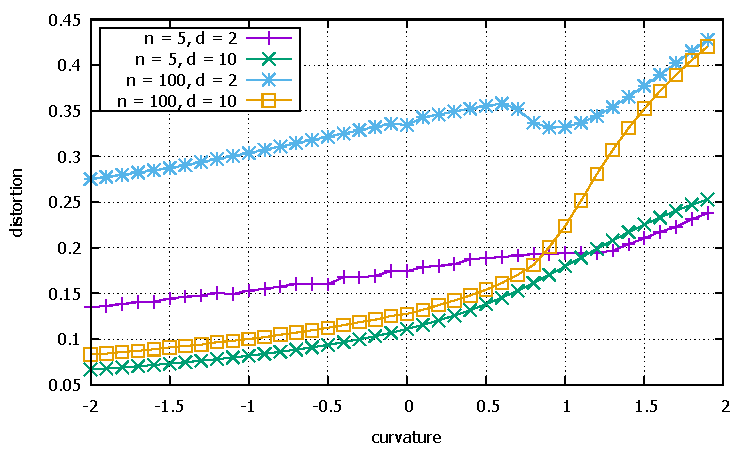
\includegraphics[width = 0.49 \textwidth]{star_distortion.pdf}
    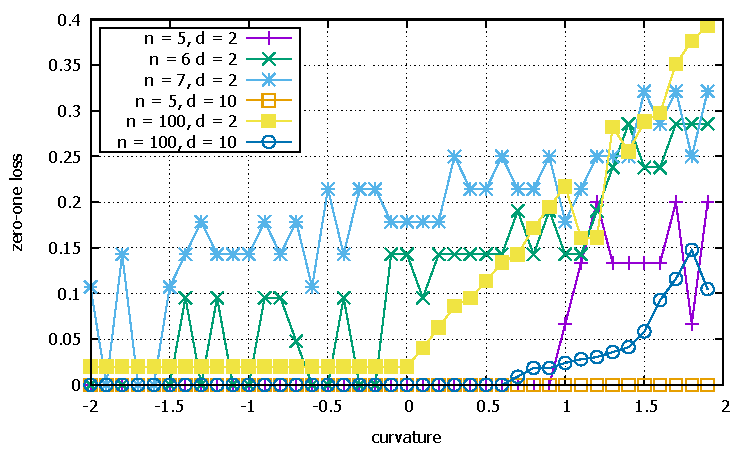
\includegraphics[width = 0.49 \textwidth]{star_zero_one.pdf}
    \caption{Star $S_n$}
    \label{fig:star}
\end{figure}

It is pointed out in numerous papers that trees are negatively curved. 
We analyze this theoretically and start with the simplest tree: one central node and $n$ \ph{leafs}. We denote this graph by $S_n$ and assume that $n \ge 3$.

\paragraph{Ollivier curvature} 
Consider any tree graph $T$, let $v, u$ be two neighbors. Then Proposition 2 in~\citep{jost2014ollivier} states that
\begin{equation}\label{eq:ollivier_tree}
	\kappa_T(u,v) = -2\left(1 - \frac{1}{\mathrm{deg}(v)} - \frac{1}{\mathrm{deg}(u)}\right)^+, 
\end{equation}
where $t^+ = \max\{0,t\}$. In particular, if either $\mathrm{deg}(v) = 1$ or $\mathrm{deg}(u) = 1$, then $\kappa_T(u,v) = 0$.  As a result, for a star we have $\kappa_{S_n}(u,v) = 0$, so $\kappa(S_n) = 0$.

\paragraph{Forman curvature}
If follows from \Eqref{eq:forman} and \Eqref{eq:forman2} that
$F(S_n) = \hat F(S_n) = 3-n$.

%\paragraph{Approximate Ollivier curvature} According to \Eqref{eq:def_ollivier_ricci_approx}, $\kappa_G^* = 0$.

\paragraph{Average sectional curvature}

Heuristic sectional curvature is defined for a node and its two neighbors. In case of a star we can only take a central node $v$ and two neighboring ones $b$ and $c$. For any other node $a$ we obtain $\xi_{S_n}(v;b,c;a) = -1$. Therefore, by averaging we obtain $\xi(S_n) = -1$.

\paragraph{Distortion-based curvature} 
We prove the following theorem (the proof is in Appendix~\ref{app:star_distortion}).
\ph{[We should be very explicit about the type of asymptotics considered in the statement of this theorem. I think it should be $c \to -\infty$. Is that correct?]}
\begin{theorem}\label{thm:star_distortion}
For any $d$, in hyperbolic space of curvature $c$ we have $D(S_n) = \Omega\left(\frac{1}{n\max(\sqrt{-c},1)}\right)$; in spherical and euclidean spaces $D(S_n) = \Omega\left(\frac{1}{n}\right)$. Also, the optimal distortion $D_{opt}(S_n) = O\left(\frac{\log n}{\sqrt{-c}}\right)$. Therefore, for any $S_n$ we have $C_d^{dist}(S_n) = -\infty$.
\end{theorem}

This result is illustrated on Figure~\ref{fig:star} (left): distortion decreases as curvature becomes smaller.

The intuition behind this result is the following: we cannot embed a star $S_3$ with zero distortion to a space of any constant curvature and any dimension, because in case of zero distortion the central node $v$ has to lie on the geodesics between all pairs of leaves, so all 4 nodes have to belong to one geodesics, which is impossible. Moreover, the same problem occurs if any graph $G$ contains $S_3$ as an induced subgraph.
On the other hand, if $c \to -\infty$, we can spread all leaves of $S_n$ uniformly on a circle of radius 1 around the central node and distortion of such construction will tend to zero since the distance between the pairs of leaves will tend to 2 (triangle become more thin). 
Further we will see that if we minimize threshold-based loss, then any tree can be perfectly embedded with $d = 2$.

\paragraph{Threshold-based curvature} 
Here we have the following theorem (the proof is in Appendix~\textcolor{red}{[todo]}).

\begin{theorem}\label{thm:star_threshold}
$C_d^{thr}(S_n) = (-\infty, C)$ for some $C = C(n,d)$, which increases with $d$ and decreases with $n$. In particular, for $d = 2$, if $n < 6$, then $C = \left(\arccos \frac{\cos \frac{2\pi}{n}}{1 - \cos \frac{2\pi}{n}}\right)^2$; if $n = 6$, then $C = 0$; if $n > 6$, then $C = - \left(2\,\mathrm{arccosh}\frac{1}{2\sin \frac{\pi}{n}}\right)^2$.
\end{theorem}

\textcolor{red}{[It would be good if we could add some bounds for $d > 2$]}

The result is illustrated on Figure~\ref{fig:star} (right). Note that zero-one loss can be noisy, especially on small graphs, since it is threshold-based, i.e., discrete.

\subsubsection{Tree $T_b$ with branching factor $b$}

\begin{figure}
    \centering
    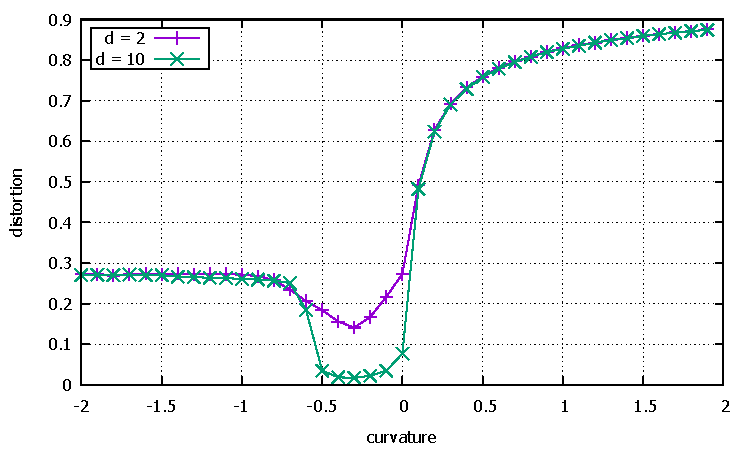
\includegraphics[width = 0.49 \textwidth]{tree_3_6_distortion.pdf}
    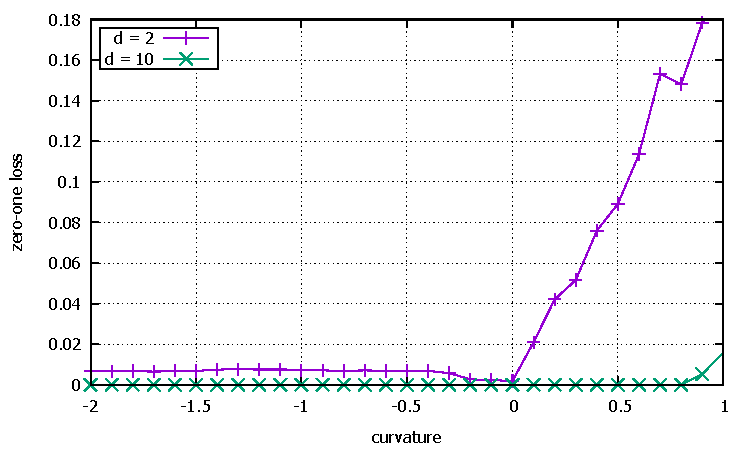
\includegraphics[width = 0.49 \textwidth]{tree_3_6_zero_one.pdf}
    \caption{Tree $T_{3,6}$ with branching factor $3$ and depth $6$}
    \label{fig:tree}
\end{figure}

We consider a tree $T_b$, $b \ge 2$. For symmetry, assume that the first node has $b+1$ children, while all other nodes have a parent and $b$ children. Also, for Ollivier, Forman and threshold based curvatures, we assume that the depth of $T_b$ is infinite. In other cases, our statements hold for any finite tree $T$.

\paragraph{Ollivier curvature} We can use \Eqref{eq:ollivier_tree} and get, for any edge,
$\kappa_{T_b}(u,v) = -2 \left(1 - \frac{1}{b+1} - \frac{1}{b+1} \right) = - 2 + \frac{4}{b+1}$. So, $\kappa(T_b) = -2 + \frac{4}{b+1}$.

\paragraph{Forman curvature} 
It is easy to see that we have 
$F(T_b) = \hat F(T_b) = 4 - 2(b+1) = 2(1-b)$.

%\paragraph{Approximate Ollivier curvature} 
%$\kappa_G^\ast(u,v) = -2 + \frac{4}{b+1}$.

\paragraph{Average sectional curvature} In contrast to Ollivier and Forman curvature, heuristic sectional curvature is global, i.e., it depends on the whole graph, which has to be finite. Note that for any tree, to compute sectional curvature, we average 0 and -1. As a result, for any tree $T$ we have $\xi(T) \in [-1,0]$. 

\textcolor{red}{[Can try to compute precisely for finite depths.]}

\paragraph{Distortion-based curvature} 

On the one hand, our result for $S_n$ implies that if a graph contains $S_3$, then it cannot be embedded with zero distortion in any space. One the other hand, \citet{sarkar2011low} proves that if we scale all edges by a sufficiently large factor $\tau$, then the obtained tree can be embedded to hyperbolic plane with distortion at most $1 + \varepsilon$ with arbitrary small $\varepsilon$. Note that multiplying graph edges by $\tau$ is equivalent to changing curvature from $1$ to $\tau^2$. As a result, \citet{sarkar2011low} proves that we can achieve arbitrary small distortion if $c \to -\infty$.
Hence, $C_d^{dist}(T) = -\infty$ for any $T$.

\textcolor{red}{[Refer to Figure~\ref{fig:tree} (left), explain the difference with theory (bad algorithm or precision problem). Alternatively~--- remove the figure.]}

\paragraph{Threshold-based curvature} 

We prove the following theorem (see Appendix~\textcolor{red}{[todo]}).

\begin{theorem}\label{thm:tree_threshold}
$C_d^{thr}(T_b) = (-\infty, C)$ for some $C = C(b,d)$, which increases with $d$ and decreases with $b$. 
The following lower bound holds: $C \ge \left( \frac{\log b}{2 \, \mathrm{arccosh} \frac{\cosh 1}{\cosh 1/2} - 1} \right)^2$.
\end{theorem}

\textcolor{red}{[It is also doable to prove the upper bound, but I don't have time to do it now, want to finish other things first.]}

Figure~\ref{fig:tree} (right) illustrates the above theorem.

\subsubsection{Complete graph $K_n$}

\begin{figure}
    \centering
    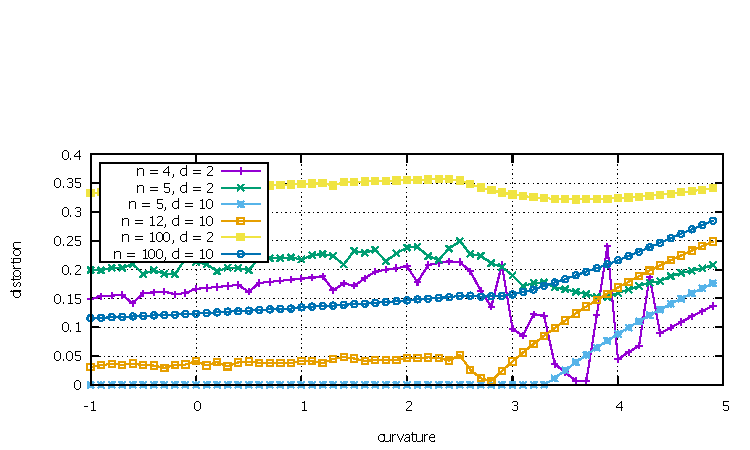
\includegraphics[width = 0.8 \textwidth]{clique_distortion.pdf}
    \caption{Complete graph $K_n$}
    \label{fig:clique}
\end{figure}

\paragraph{Ollivier curvature}  
For any two nodes $u$ and $v$, it follows from Example 1 in~\citep{jost2014ollivier} that $\kappa_{K_n}(v, u) = \frac{n-2}{n-1}$. Thus, $\kappa(K_n) = \frac{n-2}{n-1}$ and it tends to 1 as $n \to \infty$.

\paragraph{Forman curvature} 
Simple computations yield:
$F(K_n) = 6 - 2n$, $F_2(K_n) = n$.

\paragraph{Heuristic sectional curvature} 
$\xi(K_n) = \frac{1}{8}$.

\paragraph{Distortion-based curvature}

It is easy to find $C_d^{dist}(K_n)$ for $d = n-2$, since in this case there is a unique sphere with zero embedding (see Appendix~\textcolor{red}{todo}). Also, for any $d$ and $n$ if $c \to -\infty$, then optimal distortion tends to zero.

\begin{theorem}\label{thm:clique_distortion}
$C_{n-2}^{dist}(K_n) = \bigg\{-\infty,  4 \left(\arcsin \sqrt{\frac{n}{2(n-1)}}\right)^2\bigg\}$.
\end{theorem}

This result is illustrated on Figure~\ref{fig:clique}. For $n = 4, d = 2$ we expect to see the minimum at about $3.65$, for $n = 12, d = 2$ we expect $2.76$, which is indeed the case. For other parameters we do not have theoretical results, however we see sudden drops in positive curvature. Finally, as expected, distortion decreases as curvature becomes small. 

\paragraph{Threshold-based curvature} 
$C_d^{thr}(K_n) = \R$, since we can embed any complete graph perfectly by mapping all nodes to one point. 

\subsubsection{Cycle graph $C_n$} 

\begin{figure}
    \centering
    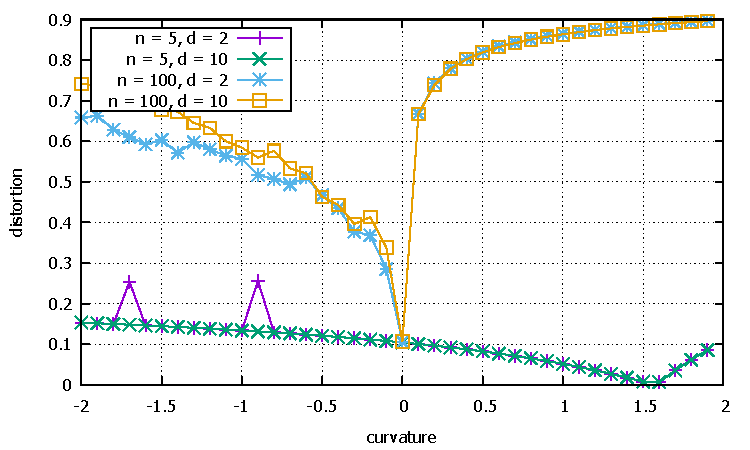
\includegraphics[width = 0.49 \textwidth]{cycle_distortion.pdf}
    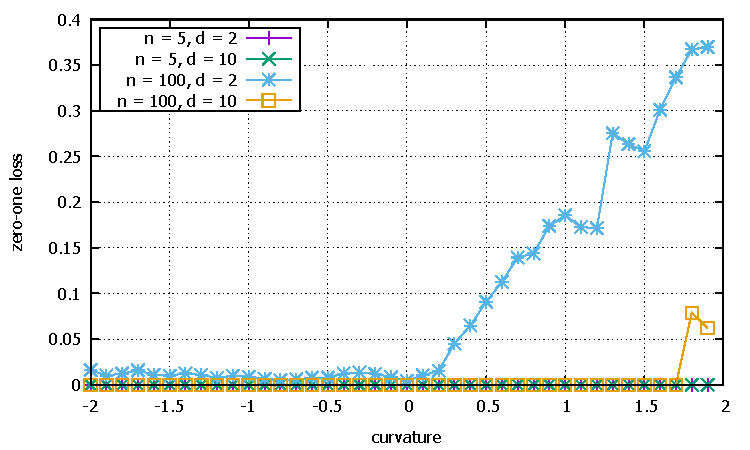
\includegraphics[width = 0.49 \textwidth]{cycle_zero_one.pdf}
    \caption{Cycle graph $C_{n}$}
    \label{fig:cycle}
\end{figure}

We consider a cycle $C_n$ with $n \ge 4$.

\paragraph{Ollivier curvature}  
Let $v \sim u$ be two neighbors. Then it is easy to see that $W_1^G(m_u,m_v) = 1$ and hence $\kappa_G(u,v) = 0$. Thus, $\kappa(C_n) = 0$.

\paragraph{Forman curvature} 

Similarly, it is easy to see that $F(C_n) = \hat F(C_n) = 0$.

%\paragraph{Approximate Ollivier curvature} 
%Using \Eqref{eq:def_ollivier_ricci_approx}, we derive  $\kappa^*(C_n) = 0$.

\paragraph{Heuristic sectional curvature} If $n$ is even, then $\xi_{C_n}(v;b,c;a) = 0$ for all points except the one diametrically opposite to $v$ for which we have $\xi_{C_n}(v;b,c;a) = 1$. If $n$ is odd, then for two points we have $\xi_{C_n}(v;b,c;a) = \frac{n}{2(n-1)}$. As a result, $\xi(C_n) = \frac{1}{n-3}$ for even $n$ and $\xi(C_n) = \frac{n}{(n-1)(n-3)}$ for odd $n$.

\paragraph{Distortion-based curvature} 

\ph{[Where is the proof of this proposition?]} \lt{[Just below the proposition]}\ph{[It seems to be more of a simple observation. I would therefore suggest to not state it as a proposition.]} 
%\begin{proposition}\label{prop:cycle_distortion}
%$C_d^{dist}(C_n) = \left(\frac{2\pi}{n}\right)^2$.
%\end{proposition}
\ph{Here we have that
\begin{equation}\label{eq:cycle_distortion}
	C_d^{dist}(C_n) = \left(\frac{2\pi}{n}\right)^2.
\end{equation}
}
Indeed, if we consider any three consequent nodes, then the middle one should lie on the geodetic between the other two. So, they all lie on a great circle (of length $n$) from which the proposition follows.
In particular, $C_d^{dist}(C_5) \approx 1.58$, $C_d^{dist}(C_{100}) \approx 0.004$, which is illustrated on Figure~\ref{fig:cycle} (left).

\textcolor{red}{[also, very negative curvature wins]}

\paragraph{Threshold-based curvature} 
Here, again, we have $C_d(C_n) = (-\infty, C)$ with some $C>0$. It is easy to prove that any curvature $c < \left(\frac{4\pi}{n}\right)^2$ is ok, but I have to think whether we can get some reasonable larger bound. \textcolor{red}{[todo]}


\subsubsection{Complete bipartite graph $K_{l,m}$}

\begin{figure}
    \centering
    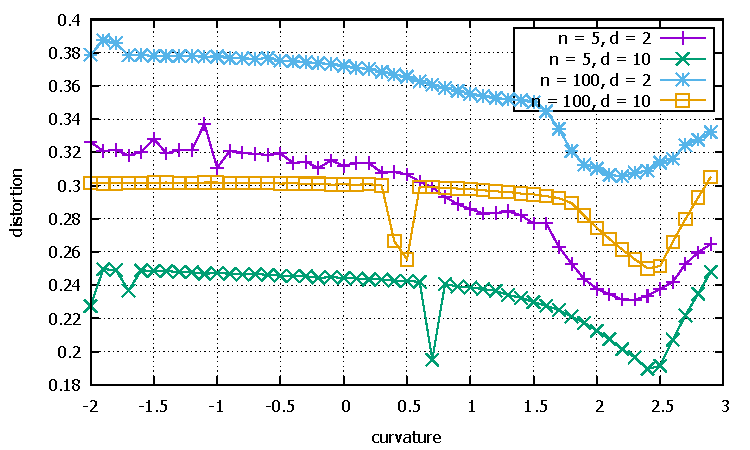
\includegraphics[width = 0.49 \textwidth]{bipartite_distortion.pdf}
    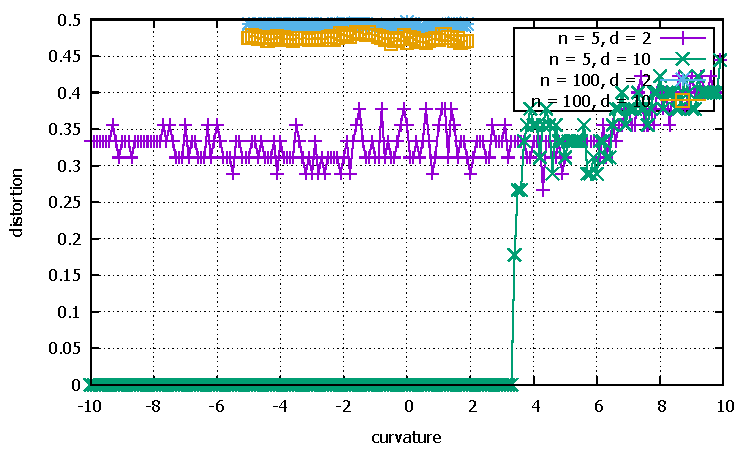
\includegraphics[width = 0.49 \textwidth]{bipartite_zero_one.pdf}
    \caption{Complete bipartite graphs $K_{n,n}$}
    \label{fig:bipartite}
\end{figure}


W.l.o.g. we assume that $l \ge m \ge 2$ (the remaining cases are stars and are already considered).

\paragraph{Ollivier curvature}  
We prove the following lemma (the proof is in Appendix~\textcolor{red}{[todo]}).

\begin{lemma}\label{lem:bipartite_ollivier}
$\kappa(K_{l,m}) = 0$.
\end{lemma}

\paragraph{Forman curvature} 

$F(K_{l,m}) = \hat F(K_{l,m}) = 4 - l - m$. Again, Forman curvature can be highly negative.

%\paragraph{Approximate Ollivier curvature} 
%In is easy to derive from \Eqref{eq:def_ollivier_ricci_approx} that $\kappa^*(K_{l,m}) = 0$. \textcolor{red}{[Which is probably significantly different from true Ollivier curvature.]}

\paragraph{Heuristic sectional curvature} If $v$ and $a$ are in the same part of the bipartite graph, then $\xi_{K_{l,m}}(v;b,c;a) = 1$, otherwise $\xi_{K_{l,m}}(v;b,c;a) = -1$. Therefore, if $a$ belongs to the part of size $l$, sectional curvature is
$\xi_{K_{l,m}}(v;b,c) = \frac{l-m+1}{l+m-3}$, otherwise it is $\xi_{K_{l,m}}(v;b,c) = \frac{m-l+1}{l+m-3}$. As a result, by averaging over all triplets, we get

\[
\xi({K_{l,m}}) = \frac{1}{l \binom{m}{2} + m \binom{l}{2}} \left(l \binom{m}{2} \frac{l-m+1}{l+m-3} + m \binom{l}{2} \frac{m-l+1}{l+m-3}\right) = \frac{-(l - m)^2 + m + l - 2}{(m+l-2)(l+m-3)}.
\]
In particular, if $m = l$ we get $\xi({K_{l,m}}) = \frac{1}{2m - 3}$. In other words, for balanced complete bipartite graphs $\xi({K_{l,m}})$ is positive, but tends to zero as graph grows.

\paragraph{Distortion-based curvature} 

Figure~\ref{fig:bipartite} (left) shows the empirical behavior of distortion depending on curvature. We observe that for all graphs optimal curvature is between 2 and 2.5. 
The following proposition gives an intuition about why one could expect this. 

\begin{proposition}\label{prop:bipartite_distortion}
For any $d$, $C_d^{dist}(K_{2,2}) = \left(\frac{\pi}{2}\right)^2 \approx 2.47$ and $K_{2,2}$ is the only complete bipartite graph (with at least two nodes in each part) for which zero distortion is achievable.
\end{proposition}

Indeed, the result for $K_{2,2}$ follows from~\Eqref{eq:cycle_distortion}. Moreover, if for $K_{l,m}$ we have $l \ge 3$ and $m \ge 2$, then for any two nodes in the part of size 3 there are at least 2 different geodesics of length 2 between them. Therefore, all such pairs lie at opposite poles of the hypersphere, which is impossible since $l \ge 3$.

\paragraph{Threshold-based curvature} 
 
Threshold-based embeddings to Euclidean spaces are well studied. In particular, it is know that for any graph $G(V,E)$ a perfect threshold embedding  exists for some $d \le |V|$~\citep{maehara1984space}. 
However, undirected bipartite graphs are hard to embed in Euclidean space: the bound $d = O(n)$ is known~\citep{maehara1984space}. We empirically observe that they are similarly hard to embed to both spherical and hyperbolic spaces, as shown on Figure~\ref{fig:bipartite} (right). Empirically, these graphs are insensitive to curvature (given it is not too large, so that a sphere is too small).
 
\section{Experiments}

\subsection{Experimental setup}

\textcolor{red}{[Describe or refer to appendix]}

\textcolor{red}{[Refer to the table with datasets in appendix]}

\textcolor{red}{[Also, mention how plots with error depending on curvature were created in all cases]}

\subsection{Comparison of curvature estimators}

\textcolor{red}{[Tables are in progress]}

\begin{table}[t]
\caption{Compare curvature estimators, distortion}
\label{tab:compare_distortion}
\begin{center}
\begin{tabular}{lcccccccccc}
&
\multicolumn{2}{c}{Ollivier} &
\multicolumn{2}{c}{Forman} &
\multicolumn{2}{c}{Avg. sectional} &
\multicolumn{2}{c}{Grad. descent} &
\multicolumn{2}{c}{Grid search} \\
Dataset/dim & c & loss  & c & loss  & c & loss  & c & loss  & c & loss \\
 \hline \\
$S_{100}$ / 2 &
0.0 & 0.334 & 
-97.0 & 0.058 & 
-1.0 & 0.304 &
& \\
%-2.0 & 0.275 \\
$S_{100}$ / 10 &
0.0 & 0.127 & 
-97.0 & 0.014 & 
-1.0 & 0.1 & 
& \\
%-2.0 & 0.083\\
$T_{3,6}$ / 2 &
-0.33 & 0.136 & 
-2.0 & 0.254 & 
-0.5 & 0.174 & 
& \\
%-0.2 & 0.141 \\
$T_{3,6}$ / 10 &
-0.33 & 0.016 & 
-2.0 & 0.243 & 
-0.5 & 0.036 & 
& \\
%-0.2 & 0.017 \\
$K_{100}$ / 2 & 
0.99 & 0.348 & 
100 & 0.841 & 
0.125 & 0.342 & 
& \\
%3.6 & 0.322 \\
$K_{100}$ / 10 & 
0.99 & 0.134 & 
100 & 0.841 & 
0.125 & 0.124 & 
& \\
%-1.9 & 0.108 \\
$C_{100}$ / 2 & 
0.0 & 0.106 & 
0.0 & 0.106 & 
0.01 & 0.257 &
& \\
%0.0 & 0.106 \\
$C_{100}$ / 10 & 
0.0 & 0.106 & 
0.0 & 0.106 & 
0.01 & 0.255 & 
& \\
%0.0 & 0.106 \\
$K_{100,100}$ / 2 &
0.0 & 0.372 & 
-196 & 0.294 & 
0.008 & 0.372 & 
& \\
%2.2 & 0.306 \\
$K_{100,100}$ / 10 &
0.0 & 0.301 & 
-196 & 0.275 & 
0.008 & 0.301 & 
& \\
%2.4 & 0.250 \\
Karate / 2 &
0.01 & 0.197 & 
-6.35 & 0.248 &
0.30 & 0.206 &
& \\
%-1.8 & 0.160 \\
Karate / 10 &
0.01 & 0.105 & 
-6.35 & 0.157 &
0.30 & 0.126 &
& \\
%-0.4 & 0.100 \\
Conflict / 2 &
-0.2 &	0.229 &
-16.5 &	0.261 &
0.25 & 	0.269 &
& \\
Conflict / 10 &
-0.2 & 0.078 &
-16.5 &	0.243 &
0.25 &	0.173 &
& \\
Chicago / 2 &
-0.19 & 0.225 & 
-8.37 & 0.224 & 
-0.6 & 0.178 & 
& \\
Chicago / 10 &
-0.19 & 0.045 & 
-8.37 & 0.216 & 
-0.6 & 0.024 & 
& \\
CSPhDs / 2 &
-0.28 &	0.152 &
-7.92 &	0.420 &
-0.26 & 0.172 &
& \\
CSPhDs / 10 &
-0.28 &	0.085 &
-7.92 &	0.412 &
-0.26 & 0.208 &
& \\
Euroroad / 2 &
-0.36 &	0.267 &
-1.95 &	0.452&
0.027 &	0.384&
& \\
Euroroad / 10 &
-0.36 &	0.264 &
-1.95 &	0.445 &
0.03 &	0.370 &
& \\
\hline \\
\end{tabular}
\end{center}
\end{table}

\begin{table}[t]
\caption{Compare curvature estimators, zero-one loss}
\label{tab:compare_zero_one}
\begin{center}
\begin{tabular}{lcccccccc}
&
\multicolumn{2}{c}{Ollivier} &
\multicolumn{2}{c}{Forman} &
\multicolumn{2}{c}{Avg. sectional} &
\multicolumn{2}{c}{Grad. descent} 
%& \multicolumn{2}{c}{Grid search} 
\\
Dataset & c & loss  & c & loss  & c & loss & c & loss  
%& c & loss 
\\
\hline \\
$S_{100}$ / 2 &
0.0 & 0.02 & 
-97.0 & 0.004 & 
-1.0 & 0.02 &
&
%& 0.0 & 0.024
\\
$T_{3,6}$ / 2 &
-0.33 & 0.006 & 
-2.0 & 0.005 & 
-0.5 & 0.005 & 
&
%& 0.0 & 0.002 
\\
$C_{100}$ / 2 & 
0.0 & 0.005 & 
0.0 & 0.005 &
0.01 & 0.009 & 
&
%& 0.0 & 0.004 
\\
$K_{100,100}$ / 2 &
0.0 & 0.496 & 
-196 & 0.491 & 
0.008 & 0.497 & 
&
%& 0.5 & 0.486 
\\
$K_{100,100}$ / 10 &
0.0 & 0.485 & 
-196 & 0.492 & 
0.008 & 0.480 & 
&
%& -0.5 & 0.466 
\\
Karate / 2 &
0.01 & 0.135 & 
-6.35 & 0.137 &
0.30 & 0.123 &
&
%&-1.5 & 0.102
\\
Conflict / 2 &
-0.2 & 0.042 &
-16.5 &	0.048 &
0.25 & 0.059 &
& \\
Conflict / 10 &
-0.2 & 0.001 &
-16.6 &	0.025 &
0.25 & $10^{-4}$
& \\
Chicago / 2 &
-0.19 & 0.004 & 
-8.37 & 0.005 & 
-0.6 & 0.004 & 
& \\
CSPhDs / 2 &
-0.28 &	0.002 &
-7.92 &	0.004 &
-0.26 & 0.002 &
& \\
Euroroad / 2 &
-0.36 &	0.002 &
-1.95 &	0.004 &
0.027 &	0.005 &
& \\
\end{tabular}
\end{center}
\end{table}

\section{Conclusion}

\textcolor{red}{[Will be added 24.09]}

%\subsubsection*{Author Contributions}

%\subsubsection*{Acknowledgments}

\bibliography{references}
\bibliographystyle{iclr2020_conference}

\appendix

\section{Geometrical properties of spaces of constant curvature}

In this section, we recall some useful equalities which will be used throughout the proofs.

In all proofs, we use notation $R$, where $R = \frac{1}{\sqrt{c}}$ in spherical space (corresponds to the radius of a sphere) and in the hyperbolic case $(c < 0)$ $R = \frac{1}{\sqrt{-c}}$ can be considered as a scaling factor compared to the space of curvature~1.

\paragraph{Law of cosines}

Let us consider a triangle with angles $A, B, C$ and the lengths of opposite sides $a, b, c$, respectively.

In Euclidean, space we have:
\[
c^2 = a^2 + b^2 - 2 \, a\, b \cos C\,.
\]
In spherical space, the first law of cosines is:
\[
\cos \frac{c}{R} =\cos \frac{a}{R} \cos \frac{b}{R} + \sin \frac{a}{R}\sin \frac{b}{R}\cos C \,,
\]
and the second law of cosines is:
\[
\cos C=-\cos A\cos B+\sin A\sin B\cos \frac{c}{R}\,.
\]

In hyperbolic space, we have 
\[
\cosh {\frac {c}{R}}= \cosh {\frac {a}{R}}\cosh {\frac {b}{R}}-\sinh {\frac {a}{R}}\sinh {\frac {b}{R}}\cos C \,.
\]

\textbf{Equilateral triangle}

The following equalities follow from the corresponding laws of cosines, assuming that all sides (and angles) are equal.

For hyperbolic space:
\begin{equation}\label{eq:hyp_eq}
\cosh\frac{a}{2R} = \frac{1}{2\sin \frac{A}{2}}\,.
\end{equation}

For spherical space:
\begin{equation}\label{eq:sph_eq}
\cos{\frac{a}{R}} = \frac{\cos A}{1 - \cos A}.
\end{equation}

\paragraph{Area and volume of hypersphere}

Let $S_d(r)$ and $V_d(r)$ denote area of a hypersphere and volume of a ball of radius $r$ in $d$-dimensional space. 

In euclidean space,
\[
S_d(r)= d \, C_{d} \, r^{d-1},
\]
\[
V_d(r)= C_{d} \, r^{d},
\]
where
\[
C_{d}={\frac  {\pi ^{{d/2}}}{\Gamma ({d \over 2}+1)}}.
\]

In spherical space, sphere of radius $r$ is isometric to Euclidean sphere of radius $R \sin \frac{r}{R}$. Therefore, the area is 
\[
S_d(r)= d \, C_{d} \, \left( R \sin \frac{r}{R} \right)^{d-1},
\]
\[
V_d(r)= d \, C_{d} \, R^d \int_{0}^{r} \left( \sin \frac{x}{R} \right)^{d-1} d x .
\]

Similarly, in hyperbolic space,
\[
S_d(r)= d \, C_{d} \, \left( R \sinh \frac{r}{R} \right)^{d-1},
\]
\[
V_d(r)= d \, C_{d} \, R^d \int_{0}^{r} \left( \sinh \frac{x}{R} \right)^{d-1} d x .
\]


\section{Ollivier curvature of simple graphs}

\subsection{Proof of Lemma~\ref{lem:bipartite_ollivier} (bipartite graphs $K_{l,m}$)}

Let use denote the node sets in $K_{l,m}$ by $U := \{u_1, \dots, u_l\}$ and $V := \{v_1, \dots, v_m\}$. We will prove that for any edge $(u, v)$, $W_1^{K_{l,m}}(m_{u},m_{v}) = 1$, which then implies that $\kappa(K_{l,m}) = 0$. 

Note that for any $u \in U, v \in V$ the joint neighborhood is $V \times U$. First we establish an upper bound by considering the product joint probability density on $V \times U$
\[
	\rho(x,y) =	\frac{1}{m l}.
\]
It then follows that
\[
	W_1^{K_{l,m}}(m_{u},m_{v}) \le \sum_{i = 1}^m \sum_{j = 1}^l d_G(v_i, u_j) \rho(v_i, u_j)
	= 1.
\]
For the lower bound we define the function
\[
	f(z) = \begin{cases}
		2 &\mbox{if } z \in V,\\
		1 &\mbox{if } z \in U.
	\end{cases}
\]
Observe that if $u \in U$ and $v \in V$ then $|f(u) - f(z)| = 1 = d_G(u,v)$. On the other hand, if $u, u^\prime \in U$ then $|f(u) - f(u^\prime)| = 0 \le 2 = d_G(u,u^\prime)$ and similar for $v, v^\prime \in V$. Thus we conclude that $f$ is 1-Lipschitz. It now follows that
\[
	W_1^{K_{l,m}}(m_u,m_v) \ge \frac{1}{m} \sum_{i = 1}^m f(v_i) - \frac{1}{l} \sum_{j = 1}^l f(u_j) = 1,
\]
which completes the proof.

\section{Distortion-based curvature of simple graphs}

\subsection{Proof of Theorem~\ref{thm:star_distortion} (star $S_n$)}\label{app:star_distortion}

The general idea is the following: we take any curvature $c$ and prove a lower bound on distortion (for any given dimension $d$). Then, we obtain an upper bound on optimal distortion which tends to zero as $c \to -\infty$, which gives the claimed result $C_d^{dist}(S_n) = -\infty$.

First, let us analyze the lower bound on distortion. Recall that distortion of a graph is the average distortion over all pairs of nodes. Let $v$ be the central node and $v_1, \ldots, v_n$ ($n \ge 3$) be its neighbors. Then, for any embedding $f$, we have
\begin{multline*}
D(S_n) = \frac{1}{\binom{n+1}{2}} \left( \sum_{v_i} {|d(f(v),f(v_i)) - 1|} + \sum_{v_i \neq v_j} \frac{|d(f(v_i),f(v_j)) - 2|}{2} \right) \\
= \frac{1}{\binom{n+1}{2}} \sum_{1 \le i_1 < i_2 < i_3 \le n} \left(
\sum_{1\le j \le 3}  \frac{|d(f(v_{i_j}),f(v)) - 1|}{{n-1 \choose 2}} +
\sum_{1\le j < k\le 3}  \frac{|d(f(v_{i_j}),f(v_{i_k})) - 2|}{2(n-2)}   \right).
\end{multline*}

Let $D_{min}$ be the minimum value of the following weighted distortion of a star with 3 leaves:
\[
D_{min} = \min_{f} \sum_{1\le j \le 3}  \frac{|d(f(v_j),f(v)) - 1|}{(n-1)/4} +
\sum_{1\le j < k\le 3}  |d(f(v_j),f(v_k)) - 2|,
\]
then 
\begin{equation}\label{eq:D_min}
D(S_n) \ge \frac{{n\choose 3}}{2(n-2){n+1 \choose 2}} D_{min} = \frac{ (n-1)D_{min}}{6(n+1)}\,.
\end{equation}
Hence, it remains to find a lower bound on $D_{min}$, i.e., a lower bound for a weighted distortion of $S_3$ with central node $v$ and three leaves $v_1, v_2, v_3$.
If we consider three angles at the node $v$, then at least one of them is $\alpha \le 2 \pi / 3$, so we can get a lower bound by only considering this triangle, which is, w.l.o.g., formed by $v, v_1, v_2$.
\[
D_{min} \ge  |d(f(v_1),f(v_2)) - 2| + \frac{|d(f(v_1),f(v)) - 1| + |d(f(v_2),f(v)) - 1|}{(n-1)/2}.
\]

Denote $d(f(v_1),f(v)) = x = 1 + \varepsilon$, $d(f(v_2),f(v)) = y = 1 + \delta$, $d(f(v_1),f(v_2)) = z = 2 + \varepsilon + \delta - \varphi$ with some $\varepsilon, \delta$ and some $\varphi > 0$ (from triangle inequality). Assume that $|\varepsilon| < 1/2$ and $|\delta| < 1/2$ (otherwise the lower bound is trivial). Now we use the law of cosines to get a lower bound on $\varphi$.
We consider Euclidean and hyperbolic spaces separately and note that the bound obtained in Euclidean space also holds in spherical spaces (with any $c$).

\textcolor{red}{In Euclidean space, using triangle inequality, we get  $\varphi = x + y - z > 0$. So, in Euclidean and spherical spaces $\varphi$ is bounded below by a constant.}
%\[
%z^2 = x^2 + y^2 - 2 x y \cos \alpha, 
%\]
%so 
%\[
%(x+y)^2 - z^2 = 2 x y \lt{(\cos \alpha+1)}.
%\]
%As $\alpha < \pi$, we get
%$\varphi = x + y - z > 0$. 

In hyperbolic space the law of cosines gives 
(recall that $R = \frac{1}{\sqrt{-c}}$):
\[
\cosh \frac{z}{R} = \cosh \frac{x}{R} \cosh \frac{y}{R} - \sinh \frac{x}{R} \sinh \frac{y}{R} \cos \alpha,
\]
from which, \lt{using $\cosh(x+y) =\cosh x\cosh y+\sinh x\sinh y$}, we get 
\[
\cosh \frac{x+y}{R} - \cosh \frac{z}{R} = \sinh \frac{x}{R} \sinh \frac{y}{R} (1 + \cos \alpha). %= \Omega\left(e^{(x+y)/R}\right).
\]
If $R \to \infty$, then, similarly to Euclidean case, we get $\varphi = x + y - z = \Omega(1)$. Otherwise, we have
\[
\cosh \frac{x+y}{R} - \cosh \frac{z}{R} = \Omega\left(e^{(x+y)/R}\right) = \Omega\left(e^{1/R}\right)
\]
and
%$e^{\frac{x+y-z}{R}} - 1 = \Omega\left(e^{\frac{x+y-z}{R}}\right) = \Omega(1)$, so 
$\varphi = x + y - z = \Omega(R)$. \ph{[I still do not follow this last step. Where does this conclusion come from and what are the asymptotics considered? It can't be $R \to \infty$ because we concluded that in that case it is bounded from below by a constant. So is it $R \to 0$?]}

Note that $D_{min} \ge |z-2| + \frac{|x-1| + |y-1|}{(n-1)/2} =  |\varepsilon + \delta - \varphi| + \frac{|\varepsilon| + |\delta|}{(n-1)/2}$. This gives us a lower bound $D_{min} = \Omega(1/n)$ in spherical and Euclidean spaces and $D_{min} = \Omega(\min(R,1)/n) = \Omega\left(\frac{1}{n\max\left(\sqrt{-c},1\right)}\right)$ in hyperbolic one. From this and \Eqref{eq:D_min} the required bound follows.

Now, let us get an upper bound on optimal distortion $D_{opt}(S_n)$. To do this, we explicitly construct an embedding with sufficiently low distortion $D(S_n)$.

Let $v$ be the central node, then we spread all other nodes uniformly on a 2-dimensional circle of radius $1$ centred at $v$. The smallest angle between two points is $2 \pi / n$. Therefore, from the law of cosines, the distance between leaves is at least $k$ with
\[
\cosh \frac{k}{R} = 1  + \left(1 -  \cos \frac{2 \pi}{n}\right)  \sinh^2 \frac{1}{R} \,.
\]

\ph{Note that for any two leaves $v_i$ and $v_j$ we have that $d(f(v_i), f(v_j)) \le 2$. In particular, the closer two leaves are, the greater the difference $2 - d(f(v_i), f(v_j))$ is. Hence, the distance between adjacent leaves is the worst case and thus $D_{opt}(S_n)$ can be upper bounded as}
%\ph{[This bound cannot be true since it only uses the distance between closest leafs]} \lt{[Do not understand this comment. The distance between closest leaves is the ``worst'' one, others are closer to two, so they give less contribution to distortion]}
\begin{multline*}
D_{opt}(S_n) \le \frac{{n \choose 2}}{2{n+1\choose 2}} \left(2 - R\cdot \mathrm{arccosh}\left( \left(1 - \cos \frac{2 \pi}{n}\right)\sinh^2\frac{1}{R}  + 1 \right)\right) \\
= \frac{(n-1)}{2(n+1)} \left(2 - R\cdot \mathrm{arccosh}\left( \left(1 - \cos \frac{2 \pi}{n}\right)\sinh^2\frac{1}{R}  + 1 \right)\right)
\end{multline*}
Note that $1 - \cos\frac{2\pi}{n} = \Theta\left(\frac{1}{n}\right)$ and $\sinh^2\left(\frac{1}{R}\right) = \Theta\left(e^{2/R}\right)$.
Then, $\textrm{arccosh}\left(\Theta\left(\frac{1}{n} e^{2/R}\right) + 1 \right)$ behaves as $\sqrt{2e^{2/R}/n}$ if $2/R \ll \log n$ and as $\frac{2}{R} - \log n$ if $2/R \gg \log n$.
Therefore, we get
\[
D_{opt}(S_n) = O\left( R \log n \right) = O\left( \frac{\log n}{\sqrt{-c}} \right).
\]

\subsection{Proof of Theorem~\ref{thm:clique_distortion} (clique $K_n$)}

\ph{[I do not understand this part. Where is the radius coming from?]}
\lt{[For simplex with side length $a$ radius of a circumscribed hypersphere is known, I took it from russian wikipedia, url is below. However, we do not need $a = 1$, we need distance on a sphere $= 1$, so I wrote the corresponding formula for this. I tried to improve the text below.]}
\url{https://ru.wikipedia.org/wiki/%D0%A1%D0%B8%D0%BC%D0%BF%D0%BB%D0%B5%D0%BA%D1%81#%D0%9E%D0%BF%D0%B8%D1%81%D0%B0%D0%BD%D0%BD%D0%B0%D1%8F_%D1%81%D1%84%D0%B5%D1%80%D0%B0}
\ph{[Is this a well-known fact? If not, then we need a reference for this.]}

If $d = n-2$, then we are given \ph{a} $(n-1)$-simplex, which can be embedded into $n-2$-dimensional spherical space. Indeed, the radius of circumscribed hypersphere for \ph{this} $(n-1)$-simplex with side length $a$ is $R = a\sqrt{\frac{n-1}{2n}}$. Since we want \ph{the} \textit{spherical} distance between all points to be equal to one, we \ph{require}
\[
\sin \frac{\alpha}{2} = \frac{a}{2R} \,\,\text{ for } \,\,\alpha = \frac{1}{R}.
\]
\ph{[It is unclear to me where this formula is coming from. Some more details would be nice.]}
\ph{This implies that
\[
2 R \arcsin \frac{a}{2R} = 1,
\]
and solving this equation for $a$ yields
%\[
%2 a\sqrt{\frac{n-1}{2n}} \arcsin \sqrt{\frac{n}{2(n-1)}} = 1,
%\]
\[
a  = \sqrt{\frac{2n}{(n-1)}}\frac{1}{2\arcsin \sqrt{\frac{n}{2(n-1)}}}.
\]
Plugging this back into the formula for the radius $R$ we obtain
\[
R = \frac{1}{2\arcsin \sqrt{\frac{n}{2(n-1)}}},
\]
so that we have
\[
C_{n-2}^{dist}(K_n) = 4 \left(\arcsin \sqrt{\frac{n}{2(n-1)}}\right)^2\,.
\]
}

\textcolor{red}{[Todo: to show that we cannot embed into space of any other curvature]}

Finally, let us show that if $c \to -\infty$, then optimal distortion $D_{opt}(K_n) \to 0$. This result follows from the fact that $D_{opt}(S_n) \to 0$, because to embed a clique, it is sufficient to embed a star on $n+1$ node with edge lengths 1/2 and then remove the central node. 

\section{Threshold-based curvature for simple graphs}

\subsection{Proof of Theorem~\ref{thm:star_threshold} (star $S_n$)}

We show below that for any $n$, any dimension $d$ and some curvature $c$ there exists a perfect embedding.
Therefore $C_d^{dist}(S_n)$ consists of curvatures for which such perfect embedding exists. 

First, let us note that if there exists a perfect embedding $f$ for some curvature $c$, then there exists a perfect embedding for any curvature $c' < c$. Indeed, w.l.o.g., we assume that the central node $v$ is mapped to the origin of a hyperspherical coordinate system and other points $v_1, \ldots, v_n$ can be described by their radii and angles. We know that the distance between $v$ and any $v_i$ is at most 1 and the distance between any pair $v_i, v_j$ is larger than one. Now we change curvature to $c' < c$ and keep hyperspherical coordinates the same. Then the distance between $v$ and any $v_i$ does not change, while the distance between nodes $v_i, v_j$ increases.

Now, it is easy to see that $C$ increases with $d$: if there exists an embedding to some dimension $d$, then, obviously, the same embedding works for $d' > d$. Further, $C$ decreases with $n$ since if there exists embedding of $S_n$, then we can easily construct an embedding of $S_{n'}$ for $n' < n$ by removing some nodes. 

Now, let us construct a perfect embedding of $S_n$
and estimate the required curvature.
Recall that in a perfect embedding all leaves have to be inside the ball of radius 1 around the central node $v$ and also the distance between any two leaves has to be larger than one. 

It is easy to see that if we managed to spread $n$ points inside the ball of radius 1 with distances more than 1 between them, then we can move each point along the radius up to distance 1 from $v$ preserving this property. Therefore, it is sufficient to spread all points on a hypersphere. 

Let us first consider $d = 2$. In this case we can find an explicit analytic expression for $C$. This will be an upper bound for any $d>2$.

First, assume that $n > 6$. In this case we have to consider only hyperbolic space, since $n$ neighbors would not fit to a circle of radius 1 in neither spherical or Euclidean spaces.

We will find such largest curvature $C$ which allows to have distance exactly 1 between the closest leaves. In this case we cannot embed $S_n$ in a space of curvature $C$, but can embed in a space of any smaller curvature. 
We use \Eqref{eq:hyp_eq} and let $\alpha = \frac{2\pi}{n}$:
%\[
%\cosh{\frac{1}{k}} = \cosh^2{\frac{1}{k}} - \sinh^2{\frac{1}{k}}\cos\alpha.
%\]
%\[
%\cosh{\frac{1}{k}} = 1 +  (1- \cos\alpha) \sinh^2{\frac{1}{k}}.
%\]
%\[
%\cosh{\frac{1}{k}} = 1 +  2\sin^2 \frac{\alpha}{2} \sinh^2{\frac{1}{k}}.
%\]
%\[
%\frac{1}{2\sin^2 \frac{\alpha}{2}} = \frac{\sinh^2{\frac{1}{k}}}{\cosh{\frac{1}{k}} - 1}.
%\]
%\[
%\frac{1}{2\sin \frac{\alpha}{2}} = \frac{\sinh{\frac{1}{k}}}{\sqrt{2}\sqrt{\cosh{\frac{1}{k}} - 1}}.
%\]
\[
\cosh\frac{1}{2R} = \frac{1}{2\sin \frac{\alpha}{2}},
\]
\[
R = \frac{1}{2\,\textrm{arccosh}\frac{1}{2\sin \frac{\alpha}{2}}},
\]
\[
C = - \left(2\,\textrm{arccosh}\frac{1}{2\sin \frac{\alpha}{2}}\right)^2.
\]

Note that if $n$ is large, then $\sin \frac{\alpha}{2} = \sin\frac{\pi}{n-1} \sim \frac{\pi}{n-1}$. Then,  $\textrm{arccosh}\frac{1}{2\sin \frac{\alpha}{2}} \sim \textrm{arccosh}\frac{n-1}{2\pi} \sim \log n$, so we get $C \sim - 4 \log^2 n$. 

Now, let us consider $n \le 6$. Obviously, for $n = 6$ we have $C = 0$.

If $n < 6$, then $C > 0$. We use \Eqref{eq:sph_eq}:
\[
\cos{\frac{1}{R}} = \frac{\cos \alpha}{1 - \cos \alpha},
\]
\[
C = \left(\arccos \frac{\cos \alpha}{1 - \cos \alpha}\right)^2.
\]

\textcolor{red}{[For $d> 2$ we can get lower and upper bounds using spherical code / kissing number, but I don't have the proofs yet.]} 

%About upper bound. If we have $n$ points at distance at least 1 from each other, then the spheres of radius 1/2 around them do no intersect. Therefore, we can find the volume that we need to get such spheres. 

%For $d > 2$ we can get lower and upper bounds for $C$. One bound we can obtain by covering the surface of a unit ball by the balls of radius $1/2$. The other bound can be obtained by using spherical packing. \textbf{[To be finished formally.]} 

\subsection{Proof of Theorem~\ref{thm:tree_threshold} (infinite tree $T_b$ with branching factor $b$)}

\textcolor{red}{[It will be good to also get upper bound here.]}

\textcolor{red}{[The proof below I wrote but did not re-read, so it can be not very detailed.]}

As for $S_n$, we prove that for $T_b$ a perfect embedding exists for $d = 2$ and some curvature $c$. Then, similarly to the previous section, it is clear that $C$ increases with $b$ and decreases with $n$.

%First, let us discuss the upper bound. 
%Here we say that all children at levels $l, l-2, l-4, \ldots$ have to fit to the ball of radius $l$ with all pairwise distances $> 1$. We can consider large enough $l$ here (and get hyperbolic space).

\begin{figure}
    \centering
    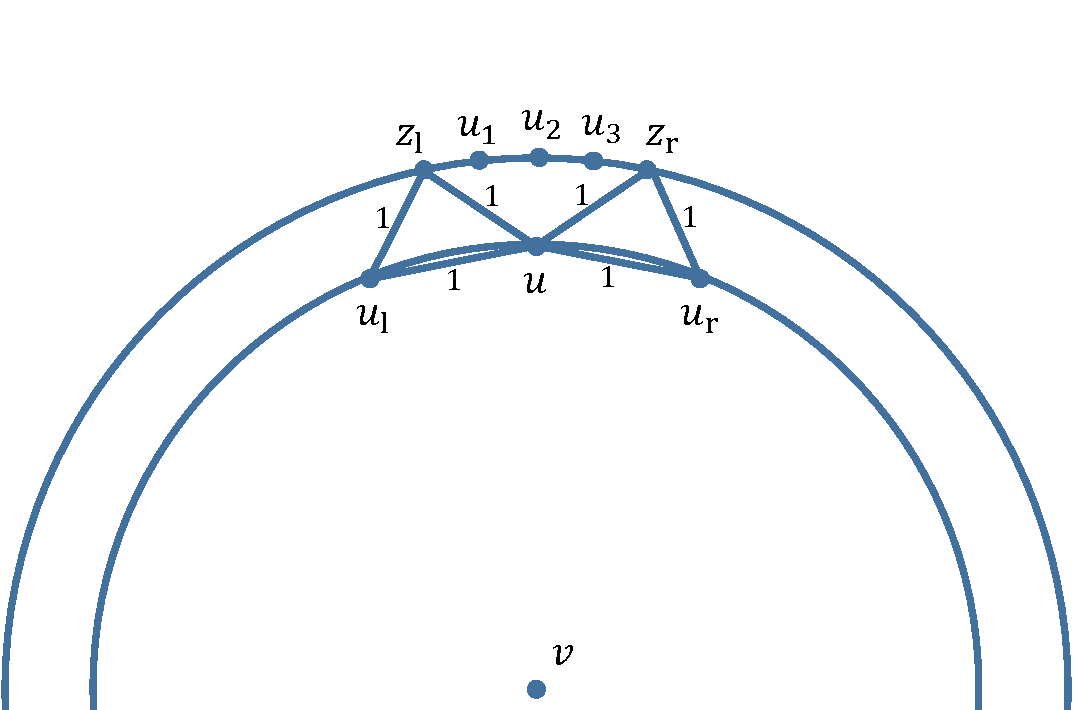
\includegraphics[width = 0.5 \textwidth]{trees.pdf}
    \caption{Threshold-based embedding of trees}
    \label{fig:trees}
\end{figure}


For the lower bound on $C$, we have to guarantee that an embedding exists. For this, we provide the following construction (see Figure~\ref{fig:trees} for an illustration).
(Below we assume that the curvature is large enough for our construction to work, then we estimate the required curvature.)
First, we take the node $v$ and consider a circle of radius 1 around this node. 
We spread $b + 1$ neighbors uniformly around this node. For our construction to work, we need all distances between these nodes to be larger than 1.
Now, at some step of the algorithm, assume that we have all nodes at level $l$ placed at some circle centered at $v$ and all distances between the nodes at level $l$ are larger than 1. Our aim is then to find positions for all nodes at level $l + 1$.

Let us take any node at $l$-th level. Consider two points $u_l$ and $u_r$ on the same circle at distance 1 from the node $u$ to the left and to the right, respectively.
Let $u,u_l,z_l$ and $u,u_r,z_r$ form equilateral triangles (with sides equal to 1). Then we let the points at $l+1$-th level to be spread on the circle centred at $v$ and passing through $z_l$ and $z_r$. The children of $u$ ($u_1, \ldots, u_{b}$) will be placed on the circular arc between $z_l$ and $z_r$. As usual, we want $u_i$ and $u_{i+1}$ to be at distance at least 1 from each other. Moreover, they have to be at distance at least 1 from children of other nodes. Also, note that placing $u_1, \ldots, u_{b}$ between $z_l$ and $z_r$ guarantees that these nodes are closer than 1 to their parent node $u$ but at the same time at a distance larger than 1 from all other nodes at $l$-th level. Also, all points at $l$-th level are far enough from points at $l+2$-th level. \ph{[Why $l+2$?]} \lt{[On level $l+1$ we already said that the neighbors are close enough and non-neighbors are far enough. However, we also now that $u$ is not connected to any node at level $l+2$ (and on all further levels).]}

It remains to find a maximum curvature such that the required conditions are satisfied. Let $r$ and $r'$ be radii of circles at $l$-th and $l+1$-th levels and let $2\alpha = \angle u_l v u$. We know (the law of cosines and $\cos 2\alpha = 1 - 2\sin^2 \alpha$) that
\begin{equation}\label{eq:1}
\cosh \frac{1}{R} = 1 + 2 \sinh \frac{r}{R} \sin^2 \alpha \,.
\end{equation}
And the only condition we need for the whole procedure to work is that we have enough space on the circular arc for placing $b$ nodes there:
\[
\cosh \frac{1}{R} \le 1 + 2 \sinh \frac{r'}{R} \sin^2 \frac{\alpha}{b} \,.
\]
Now we note that $\sin^2 \frac{\alpha}{b} \ge \frac{\sin^2 \alpha}{b^2}$ for all $b \ge 1$. Therefore, it is sufficient to have
\begin{equation}\label{eq:2}
\cosh \frac{1}{R} \le 1 + 2 \sinh \frac{r'}{R} \cdot \frac{\sin^2 \alpha}{b^2} \,.
\end{equation}
Combining \Eqref{eq:1} and \lt{\Eqref{eq:2}}, we obtain:
\[
\sinh \frac{r'}{R} \ge b^2 \cdot \sinh \frac{r}{R}.
\]
To achieve this, it is sufficient to have: \ph{[Why? I do not see this.]}
\[
\frac{r' - r}{R} \ge \log b,
\]
\[
R \le \frac{r' - r}{\log b}.
\]
It remains to find the lower bound for $r' - r$ and it is easy to see that $r' - r$ decreases with $r$. Therefore, it is sufficient to consider only the second step of the construction procedure, when we move from the circle of radius 1 to the next one. In this case, $r = 1$ and 
\[
r' = 2 \, \mathrm{arccosh} \frac{\cosh 1}{\cosh 1/2}.
\]
So, we have 
\[
-C = \frac{1}{R^2} \le \left( \frac{\log b}{2 \, \mathrm{arccosh} \frac{\cosh 1}{\cosh 1/2} - 1} \right)^2.
\]



\section{Experiments}

\subsection{Datasets}\label{sec:datasets}

Datasets used in our experiments are listed in Table~\ref{tab:datasets}. In all cases, we take only giant connection component (numbers of nodes and edges in Table~\ref{tab:datasets} correspond to already filtered dataset).

\begin{table}[t]
\caption{Dataset description}
\label{tab:datasets}
\begin{center}
\begin{tabular}{lcc}
%\multicolumn{1}{c}{\bf PART}  &\multicolumn{1}{c}{\bf DESCRIPTION}
Dataset & num. nodes & num. edges \\
 \hline \\
Karate club~\citep{zachary1977information} 
    	& 34 & 78   \\
Conflict~\citep{ward2007disputes} & 127 & 253 \\
Chicago~\citep{eash1979equilibrium} & 822 & 821 \\
CSPhDs~\citep{nooy2006exploratory} & 1025 & 1043 \\
Euroroad~\citep{vsubelj2011robust} &  1039 & 1305 \\
Power~\citep{watts1998collective} & 4941 & 6594 \\
Facebook~\cite{leskovec2012learning} & 4039 & 88234 \\
\end{tabular}
\end{center}
\end{table}

\subsection{Experimental setup}\label{sec:setup}

\subsection{Effect of curvature on real datasets}\label{sec:figures}

\textcolor{red}{[Describe our modifications and give link to code]}

\textcolor{red}{[Cite curvatures package]}

\textcolor{red}{[Describe our zero-one loss optimizer]}

See Figure~\ref{fig:karate}. \textcolor{red}{[add some conclusions]}

\begin{figure}
    \centering
    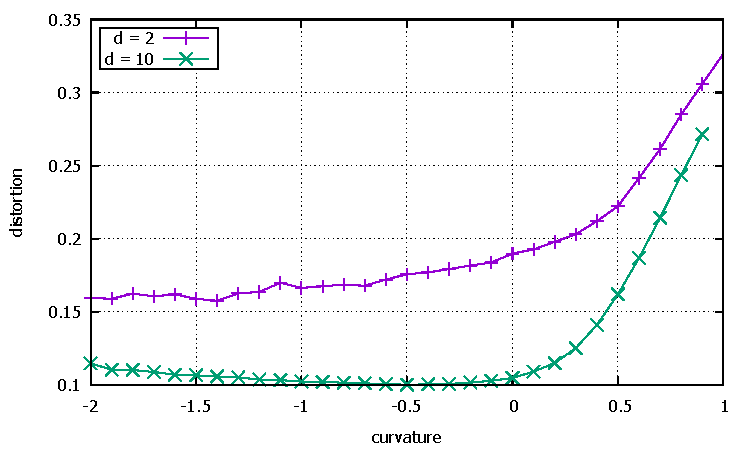
\includegraphics[width = 0.49 \textwidth]{karate_distortion.pdf}
    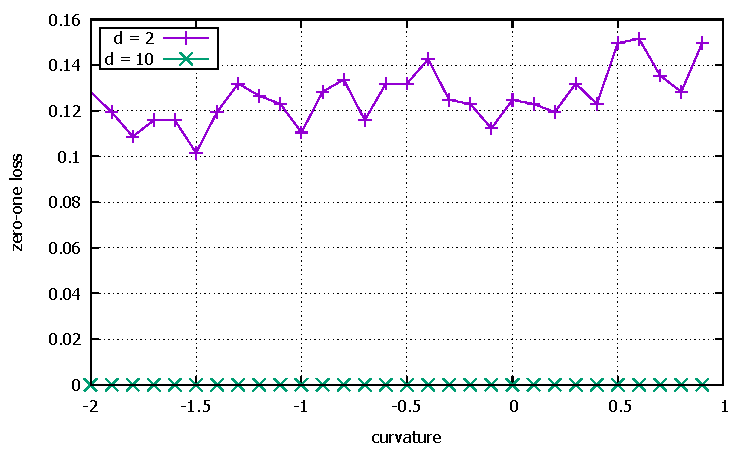
\includegraphics[width = 0.49 \textwidth]{karate_zero_one.pdf}
    \caption{Effect of curvature, Karate club dataset}
    \label{fig:karate}
\end{figure}

\begin{figure}
    \centering
    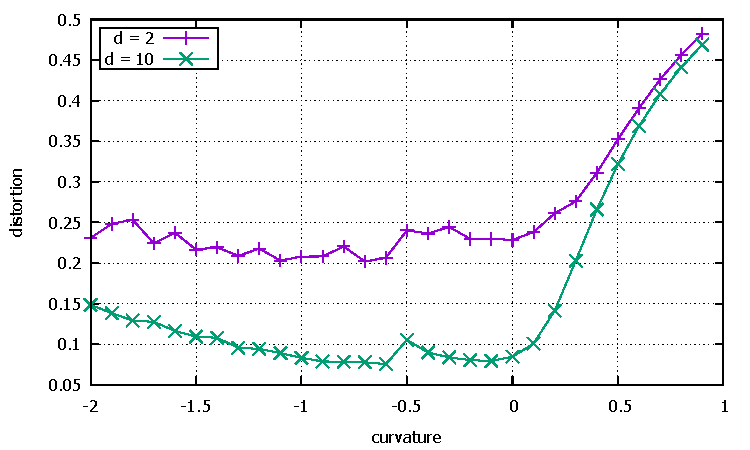
\includegraphics[width = 0.49 \textwidth]{conflict_distortion.pdf}
    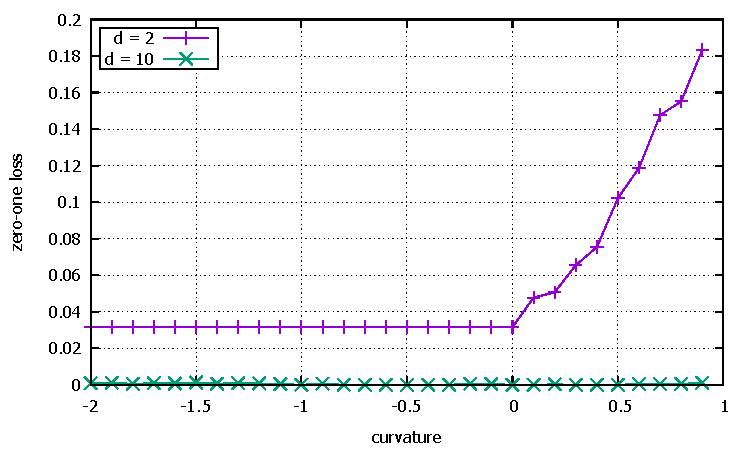
\includegraphics[width = 0.49 \textwidth]{conflict_zero_one.pdf}
    \caption{Effect of curvature, Conflict dataset}
    \label{fig:conflict}
\end{figure}

\begin{figure}
    \centering
    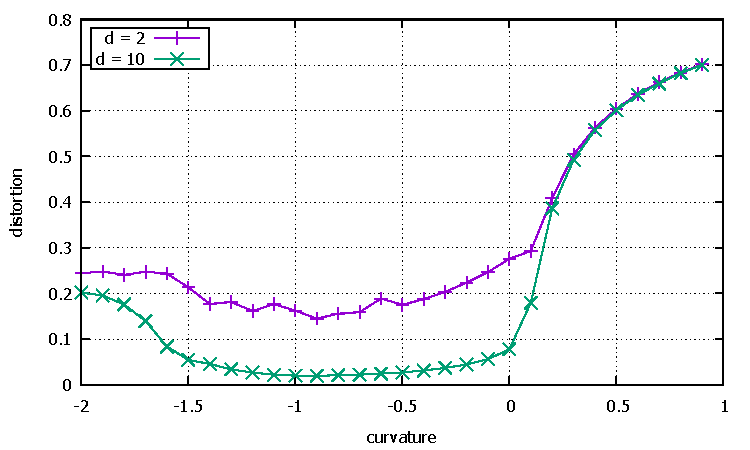
\includegraphics[width = 0.49 \textwidth]{chicago_distortion.pdf}
    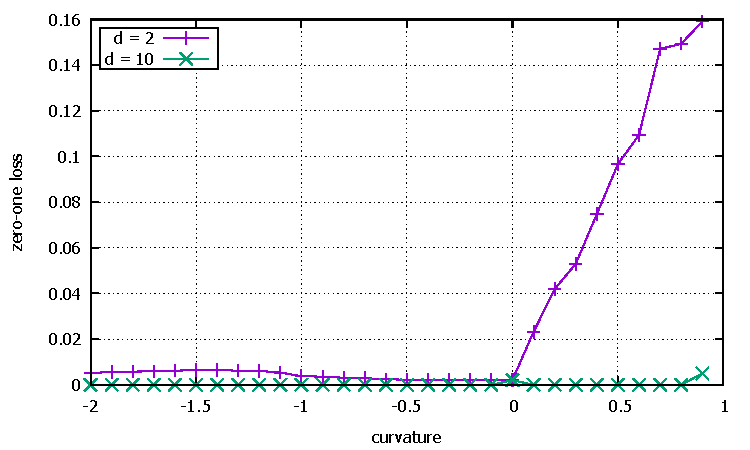
\includegraphics[width = 0.49 \textwidth]{chicago_zero_one.pdf}
    \caption{Effect of curvature, Chicago dataset}
    \label{fig:chicago}
\end{figure}

\begin{figure}
    \centering
    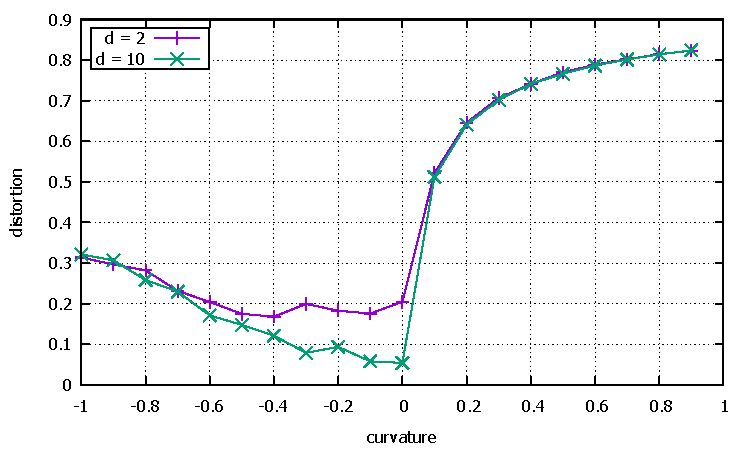
\includegraphics[width = 0.49 \textwidth]{CSPhDs_distortion.pdf}
    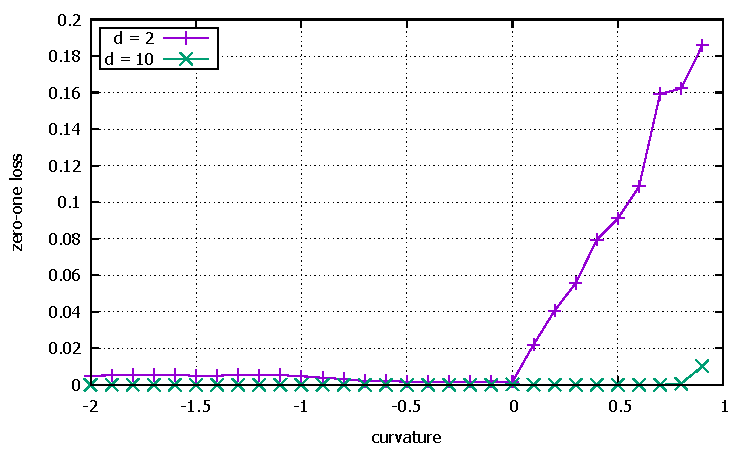
\includegraphics[width = 0.49 \textwidth]{CSPhDs_zero_one.pdf}
    \caption{Effect of curvature, CSPhDs dataset}
    \label{fig:CSPhDs}
\end{figure}

\begin{figure}
    \centering
    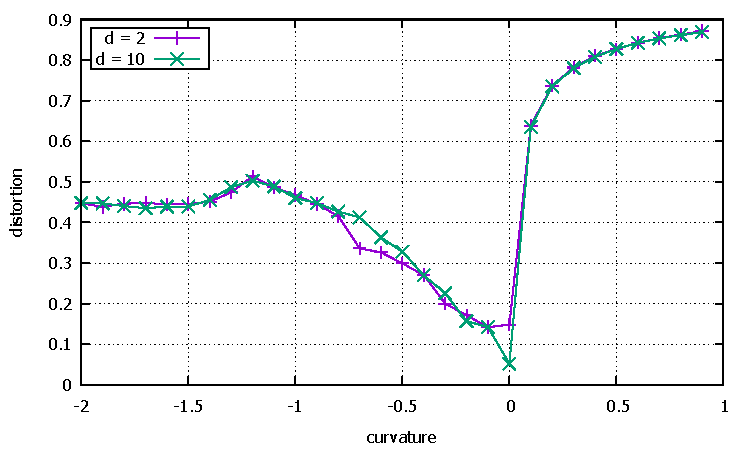
\includegraphics[width = 0.49 \textwidth]{euroroad_distortion.pdf}
    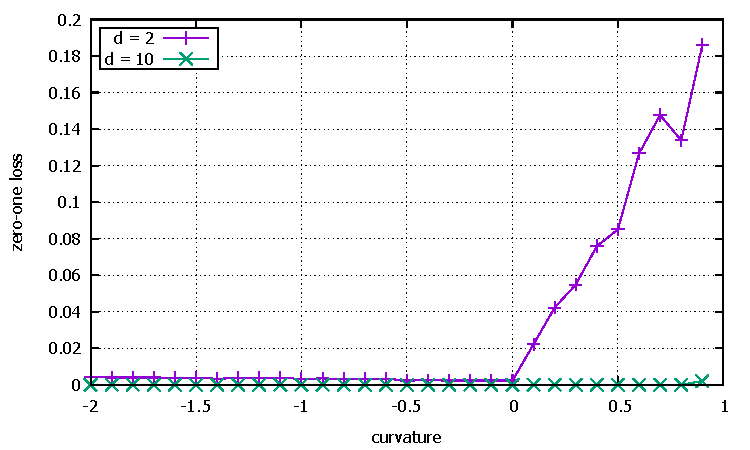
\includegraphics[width = 0.49 \textwidth]{euroroad_zero_one.pdf}
    \caption{Effect of curvature, Euroroad dataset}
    \label{fig:euroroad}
\end{figure}

\begin{figure}
    \centering
    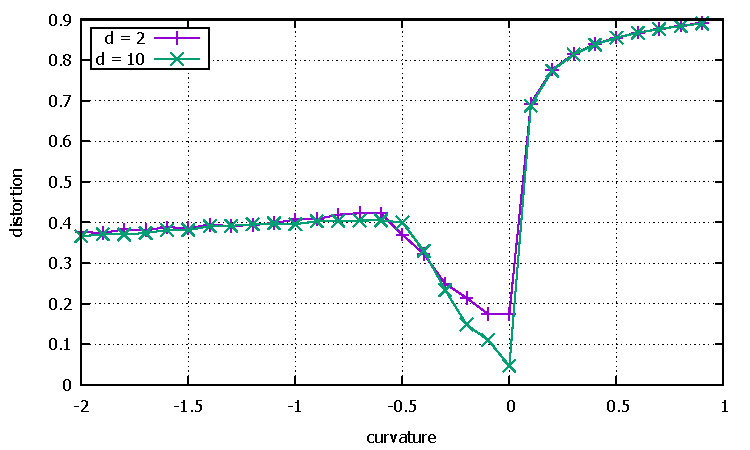
\includegraphics[width = 0.49 \textwidth]{power_distortion.pdf}
    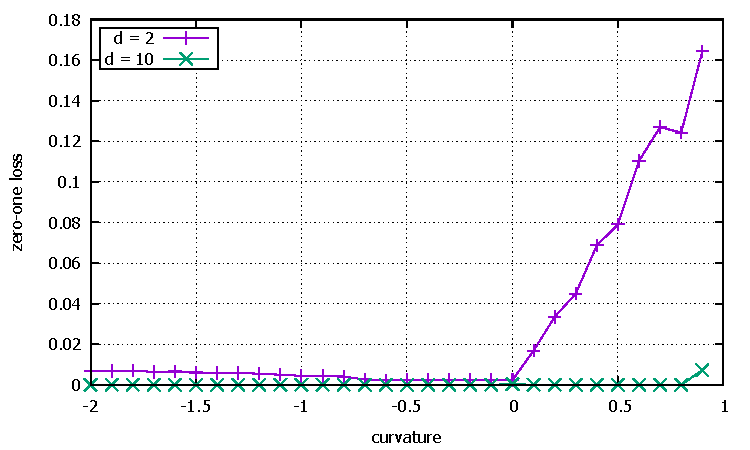
\includegraphics[width = 0.49 \textwidth]{power_zero_one.pdf}
    \caption{Effect of curvature, Power dataset}
    \label{fig:power}
\end{figure}


\end{document}





\section{Default Notation}

In an attempt to encourage standardized notation, we have included the
notation file from the textbook, \textit{Deep Learning}
\cite{goodfellow2016deep} available at
\url{https://github.com/goodfeli/dlbook_notation/}.  Use of this style
is not required and can be disabled by commenting out
\texttt{math\_commands.tex}.


\centerline{\bf Numbers and Arrays}
\bgroup
\def\arraystretch{1.5}
\begin{tabular}{p{1in}p{3.25in}}
$\displaystyle a$ & A scalar (integer or real)\\
$\displaystyle \va$ & A vector\\
$\displaystyle \mA$ & A matrix\\
$\displaystyle \tA$ & A tensor\\
$\displaystyle \mI_n$ & Identity matrix with $n$ rows and $n$ columns\\
$\displaystyle \mI$ & Identity matrix with dimensionality implied by context\\
$\displaystyle \ve^{(i)}$ & Standard basis vector $[0,\dots,0,1,0,\dots,0]$ with a 1 at position $i$\\
$\displaystyle \text{diag}(\va)$ & A square, diagonal matrix with diagonal entries given by $\va$\\
$\displaystyle \ra$ & A scalar random variable\\
$\displaystyle \rva$ & A vector-valued random variable\\
$\displaystyle \rmA$ & A matrix-valued random variable\\
\end{tabular}
\egroup
\vspace{0.25cm}

\centerline{\bf Sets and Graphs}
\bgroup
\def\arraystretch{1.5}

\begin{tabular}{p{1.25in}p{3.25in}}
$\displaystyle \sA$ & A set\\
$\displaystyle \R$ & The set of real numbers \\
$\displaystyle \{0, 1\}$ & The set containing 0 and 1 \\
$\displaystyle \{0, 1, \dots, n \}$ & The set of all integers between $0$ and $n$\\
$\displaystyle [a, b]$ & The real interval including $a$ and $b$\\
$\displaystyle (a, b]$ & The real interval excluding $a$ but including $b$\\
$\displaystyle \sA \backslash \sB$ & Set subtraction, i.e., the set containing the elements of $\sA$ that are not in $\sB$\\
$\displaystyle \gG$ & A graph\\
$\displaystyle \parents_\gG(\ervx_i)$ & The parents of $\ervx_i$ in $\gG$
\end{tabular}
\vspace{0.25cm}


\centerline{\bf Indexing}
\bgroup
\def\arraystretch{1.5}

\begin{tabular}{p{1.25in}p{3.25in}}
$\displaystyle \eva_i$ & Element $i$ of vector $\va$, with indexing starting at 1 \\
$\displaystyle \eva_{-i}$ & All elements of vector $\va$ except for element $i$ \\
$\displaystyle \emA_{i,j}$ & Element $i, j$ of matrix $\mA$ \\
$\displaystyle \mA_{i, :}$ & Row $i$ of matrix $\mA$ \\
$\displaystyle \mA_{:, i}$ & Column $i$ of matrix $\mA$ \\
$\displaystyle \etA_{i, j, k}$ & Element $(i, j, k)$ of a 3-D tensor $\tA$\\
$\displaystyle \tA_{:, :, i}$ & 2-D slice of a 3-D tensor\\
$\displaystyle \erva_i$ & Element $i$ of the random vector $\rva$ \\
\end{tabular}
\egroup
\vspace{0.25cm}


\centerline{\bf Calculus}
\bgroup
\def\arraystretch{1.5}
\begin{tabular}{p{1.25in}p{3.25in}}
% NOTE: the [2ex] on the next line adds extra height to that row of the table.
% Without that command, the fraction on the first line is too tall and collides
% with the fraction on the second line.
$\displaystyle\frac{d y} {d x}$ & Derivative of $y$ with respect to $x$\\ [2ex]
$\displaystyle \frac{\partial y} {\partial x} $ & Partial derivative of $y$ with respect to $x$ \\
$\displaystyle \nabla_\vx y $ & Gradient of $y$ with respect to $\vx$ \\
$\displaystyle \nabla_\mX y $ & Matrix derivatives of $y$ with respect to $\mX$ \\
$\displaystyle \nabla_\tX y $ & Tensor containing derivatives of $y$ with respect to $\tX$ \\
$\displaystyle \frac{\partial f}{\partial \vx} $ & Jacobian matrix $\mJ \in \R^{m\times n}$ of $f: \R^n \rightarrow \R^m$\\
$\displaystyle \nabla_\vx^2 f(\vx)\text{ or }\mH( f)(\vx)$ & The Hessian matrix of $f$ at input point $\vx$\\
$\displaystyle \int f(\vx) d\vx $ & Definite integral over the entire domain of $\vx$ \\
$\displaystyle \int_\sS f(\vx) d\vx$ & Definite integral with respect to $\vx$ over the set $\sS$ \\
\end{tabular}
\egroup
\vspace{0.25cm}

\centerline{\bf Probability and Information Theory}
\bgroup
\def\arraystretch{1.5}
\begin{tabular}{p{1.25in}p{3.25in}}
$\displaystyle P(\ra)$ & A probability distribution over a discrete variable\\
$\displaystyle p(\ra)$ & A probability distribution over a continuous variable, or over
a variable whose type has not been specified\\
$\displaystyle \ra \sim P$ & Random variable $\ra$ has distribution $P$\\% so thing on left of \sim should always be a random variable, with name beginning with \r
$\displaystyle  \E_{\rx\sim P} [ f(x) ]\text{ or } \E f(x)$ & Expectation of $f(x)$ with respect to $P(\rx)$ \\
$\displaystyle \Var(f(x)) $ &  Variance of $f(x)$ under $P(\rx)$ \\
$\displaystyle \Cov(f(x),g(x)) $ & Covariance of $f(x)$ and $g(x)$ under $P(\rx)$\\
$\displaystyle H(\rx) $ & Shannon entropy of the random variable $\rx$\\
$\displaystyle \KL ( P \Vert Q ) $ & Kullback-Leibler divergence of P and Q \\
$\displaystyle \mathcal{N} ( \vx ; \vmu , \mSigma)$ & Gaussian distribution %
over $\vx$ with mean $\vmu$ and covariance $\mSigma$ \\
\end{tabular}
\egroup
\vspace{0.25cm}

\centerline{\bf Functions}
\bgroup
\def\arraystretch{1.5}
\begin{tabular}{p{1.25in}p{3.25in}}
$\displaystyle f: \sA \rightarrow \sB$ & The function $f$ with domain $\sA$ and range $\sB$\\
$\displaystyle f \circ g $ & Composition of the functions $f$ and $g$ \\
  $\displaystyle f(\vx ; \vtheta) $ & A function of $\vx$ parametrized by $\vtheta$.
  (Sometimes we write $f(\vx)$ and omit the argument $\vtheta$ to lighten notation) \\
$\displaystyle \log x$ & Natural logarithm of $x$ \\
$\displaystyle \sigma(x)$ & Logistic sigmoid, $\displaystyle \frac{1} {1 + \exp(-x)}$ \\
$\displaystyle \zeta(x)$ & Softplus, $\log(1 + \exp(x))$ \\
$\displaystyle || \vx ||_p $ & $\normlp$ norm of $\vx$ \\
$\displaystyle || \vx || $ & $\normltwo$ norm of $\vx$ \\
$\displaystyle x^+$ & Positive part of $x$, i.e., $\max(0,x)$\\
$\displaystyle \1_\mathrm{condition}$ & is 1 if the condition is true, 0 otherwise\\
\end{tabular}
\egroup
\vspace{0.25cm}


\paragraph{Circle}

Consider a circle on $n$ nodes and let $v \sim u$ be two neighbors. Then $W_1^G(m_u,m_v) = 1$ and hence $\kappa_G(u,v) = 0$.



\paragraph{Lattice}
Consider the $2$-dimensional lattice $\mathbb{Z}^2$ and let $v \sim u$ be two neighbors. Then the optimal transportation from $m_u$ to $m_v$ is given by a translation by the vector $y - x$ and hence $W_1^G(m_v,m_u) = d_G(u,v) = 1$, see also \cite[Example 5]{ollivier2009ricci}, and thus $\kappa_G(u,v) = 0$.

\paragraph{Complete graph}

Consider a complete graph on $n$ nodes. Then, for any two nodes $u$ and $v$ it follows from Example 1 in~\cite{jost2014ollivier} that $\kappa_G(m_v, m_u) = \frac{n-2}{n-1} \to 1$ as $n \to \infty$.

\paragraph{Erd\H{o}s-Renyi graph}

The following results from~\cite{lin2011ricci} characterize Ollivier-Ricci curvature in $G(n,p)$:

\begin{enumerate}
\item If $p \ge \log(n)^{1/3} n^{-1/3}$ then almost surely
\[
	\kappa_G(u,v) = p + O\left(\sqrt{\frac{\log(n)}{n p}}\right).
\]
\item If $2 \log(n)^{1/2} n^{-1/2} \le p < \log(n)^{1/3} n^{-1/3}$ then almost surely
\[
	\kappa_G(u,v) = O\left(\frac{\log(n)}{n p^2}\right).
\]
\item If $\log(n)^{1/2} n^{-2/3} \ll p \ll \log(n)^{-1/2}$ then almost surely
\[
	\kappa_G(u,v) = -1 + O\left(n p^2\right) + O\left(\frac{\log(n)}{n^2 p^3}\right).
\]
\item If $\log(n) n^{-1} \ll p \ll n^{-2/3}$ then almost surely
\[
	\kappa_G(u,v) = -2 + O\left(n^2 p^3\right) + O\left(\sqrt{\frac{\log(n)}{np}}\right)
\]
\end{enumerate}